%%==================================================
%% thesis.tex
%%==================================================

%\documentclass[doctor, adobefonts, openright, twoside, cs4size]{sjtuthesis}
 \documentclass[bachelor, adobefonts, openright,twoside, cs4size]{sjtuthesis}
% \documentclass[master, adobefonts, review]{sjtuthesis} 
% \documentclass[%
%   bachelor|master|doctor,	% 必选项
%   adobefonts|winfonts,  	% 只测试了adobefonts,请使用adobefonts
%   oneside|twoside,		% 单面打印,双面打印(奇偶页交换页边距,默认)
%   openany|openright, 		% 可以在奇数或者偶数页开新章|只在奇数页开新章(默认)
%   cs4size|c5size, 		% 正文字号:小四、五号(默认)
%   review,	 		% 盲审论文,隐去作者姓名、学号、导师姓名、致谢、发表论文和参与的项目
%   submit			% 定稿提交的论文,插入签名扫描版的原创性声明、授权声明 
% ]
% 逐个导入参考文献数据库
\addbibresource{bib/fat.bib}
%\addbibresource{bib/thesis.bib}
%mkbibemph
%\bibliographystyle{nwpu.bst}

\begin{document}

%% 无编号内容:中英文论文封面、授权页
\title{基于微处理器的FAT32文件接口}
\author{蒲\quad{}思\quad{}行}
\advisor{陶\quad{}林\quad{}伟}
% \coadvisor{某某教授}
\defenddate{2015年6月18日}
\school{西北工业大学}
\institute{航海学院}
\studentnumber{2011300803}
\major{水声工程}

\englishtitle{The Interface of FAT32 File System Based on Microcontroller}
\englishauthor{\textsc{Pu Sihang}}
\englishadvisor{Associate Prof. \textsc{Tao Linwei}}
% \englishcoadvisor{Prof. \textsc{Uom Uom}}
\englishschool{Northwestern Polytechnical University}
\englishinstitute{\textsc{Depart of Electronics and Information, School of Marine Science and Technology} \\
  \textsc{Northwestern Polytechnical University} \\
  \textsc{ShaanXi, P.R.China}}
\englishmajor{Underwater Acoustic Engineering}
\englishdate{June, 2015}


%\maketitle
%%%%%%%%%%%%%%%%%%%%%%%%%%%%%%%%%%%%%%%%%%%%%%%%%%%%%%%%%%%%%%%%%%%%%%%%%
%
%   LaTeX File for Doctor (Master) Thesis of Tsinghua University
%   LaTeX + CJK     清华大学博士(硕士)论文模板
%   Based on Wang Tianshu's Template for XJTU
%   Version: 1.00
%   Last Update: 2003-09-12
%
%%%%%%%%%%%%%%%%%%%%%%%%%%%%%%%%%%%%%%%%%%%%%%%%%%%%%%%%%%%%%%%%%%%%%%%%%
%   Copyright 2002-2003  by  Lei Wang (BaconChina)       (bcpub@sina.com)
%%%%%%%%%%%%%%%%%%%%%%%%%%%%%%%%%%%%%%%%%%%%%%%%%%%%%%%%%%%%%%%%%%%%%%%%%
%   Changed by Benny Pu
% Make a Cover

\begin{titlepage}
\voffset 2.7cm
\begin{center}
\begin{center}
\begin{minipage}[c]{2.64cm}
\centering
\resizebox{!}{0.9cm}{%
\parbox{0.54cm}{\begin{tikzpicture}
  \draw[line width=0.1cm] (0,0) circle (2cm);
  \draw[line width=0.05cm] (0,0) circle (1.3cm);
  \fill[gray!15] (0,0) circle (1.3cm);
  \fill[white] (0,0) circle (0.9cm);
  \draw[line width=0.05cm] (0,0) circle (0.9cm);
  \fill[black] (-0.5,-0.73) .. controls (-0.35,-0.81) ..
	(-0.2,-0.8)  .. controls (0.15, -0.7) and (0.20,-0.60) .. 
	(0.35,-0.35)   .. controls (0.42, -0.24) and (0.6,-0.26) ..
	(0.6,-0.4)   .. controls (0.58,-0.50) and (0.49, -0.50) ..
	(0.45,-0.45) .. controls (0.4,-0.68) and (0.75, -0.7) ..
	(0.9,0) arc (360:250:0.9cm);
  \fill (-0.4,-0.4)--(-1.33,-0.4)--(1,1.1)--cycle;
  \fill (-0.37,-0.43)--(-0.2,-0.8)--(1.01,1.05)--cycle;
  
  \foreach \x/\txt in {0/N,1/O,2/R,3/T,4/H,5/W,6/E,7/S,8/T,9/E,10/R,11/N,12/~,13/P,14/O,15/L,16/Y,17/T,18/E,19/C,20/H,21/N,22/I,23/C,24/A,25/L,26/~,27/U,28/N,29/I,30/V,31/E,32/R,33/S,34/I,35/T,36/Y}
  {
    \node[scale=0.7,rotate=\x*-6.5-245] at (207+\x*-6.5:1.6cm) {\txt};
  };
  \foreach \x/\txt in {0/西,1/北,2/工,3/业,4/大,5/学}
  {
    \node[scale=1.25,rotate=\x*18-50] at (225+\x*18:1.65cm) {\nwpulogo\txt};
  };
  \foreach \x/\txt in {0/1,1/9,2/3,3/8}
  {
    \node[scale=1,rotate=\x*18-25] at (\x*18-115:1.1cm) {\bfseries\txt};
  };

\end{tikzpicture}
}
}
\end{minipage}
\hskip 0.8cm
\begin{minipage}[c]{8cm}
\fontsize{33}{33}\nwpulogo 西北工业大学
\end{minipage}
\end{center}
\vskip 0.7cm
\chuhao\song {\bfseries 本科毕业设计论文}
\vskip 5cm
{
\sanhao\hei 题~~目 \hspace{0.2cm}\coverunderline[12.5cm]{基于微处理器的FAT32文件接口}
}
\vskip 2cm
{
\sihao\song 专业名称\coverunderline[7cm]{水声工程}
\vskip 0.7cm
\sihao\song 学生姓名\coverunderline[7cm]{蒲~~思~~行}
\vskip 0.7cm
\sihao\song 指导教师\coverunderline[7cm]{陶~~林~~伟}
\vskip 0.7cm
\sihao\song 毕业时间\coverunderline[7cm]{2015年06月}
\vfill
}
\end{center}
\end{titlepage}

\song \normalsize





%\makeenglishtitle

\makeatletter
\ifsjtu@submit\relax
	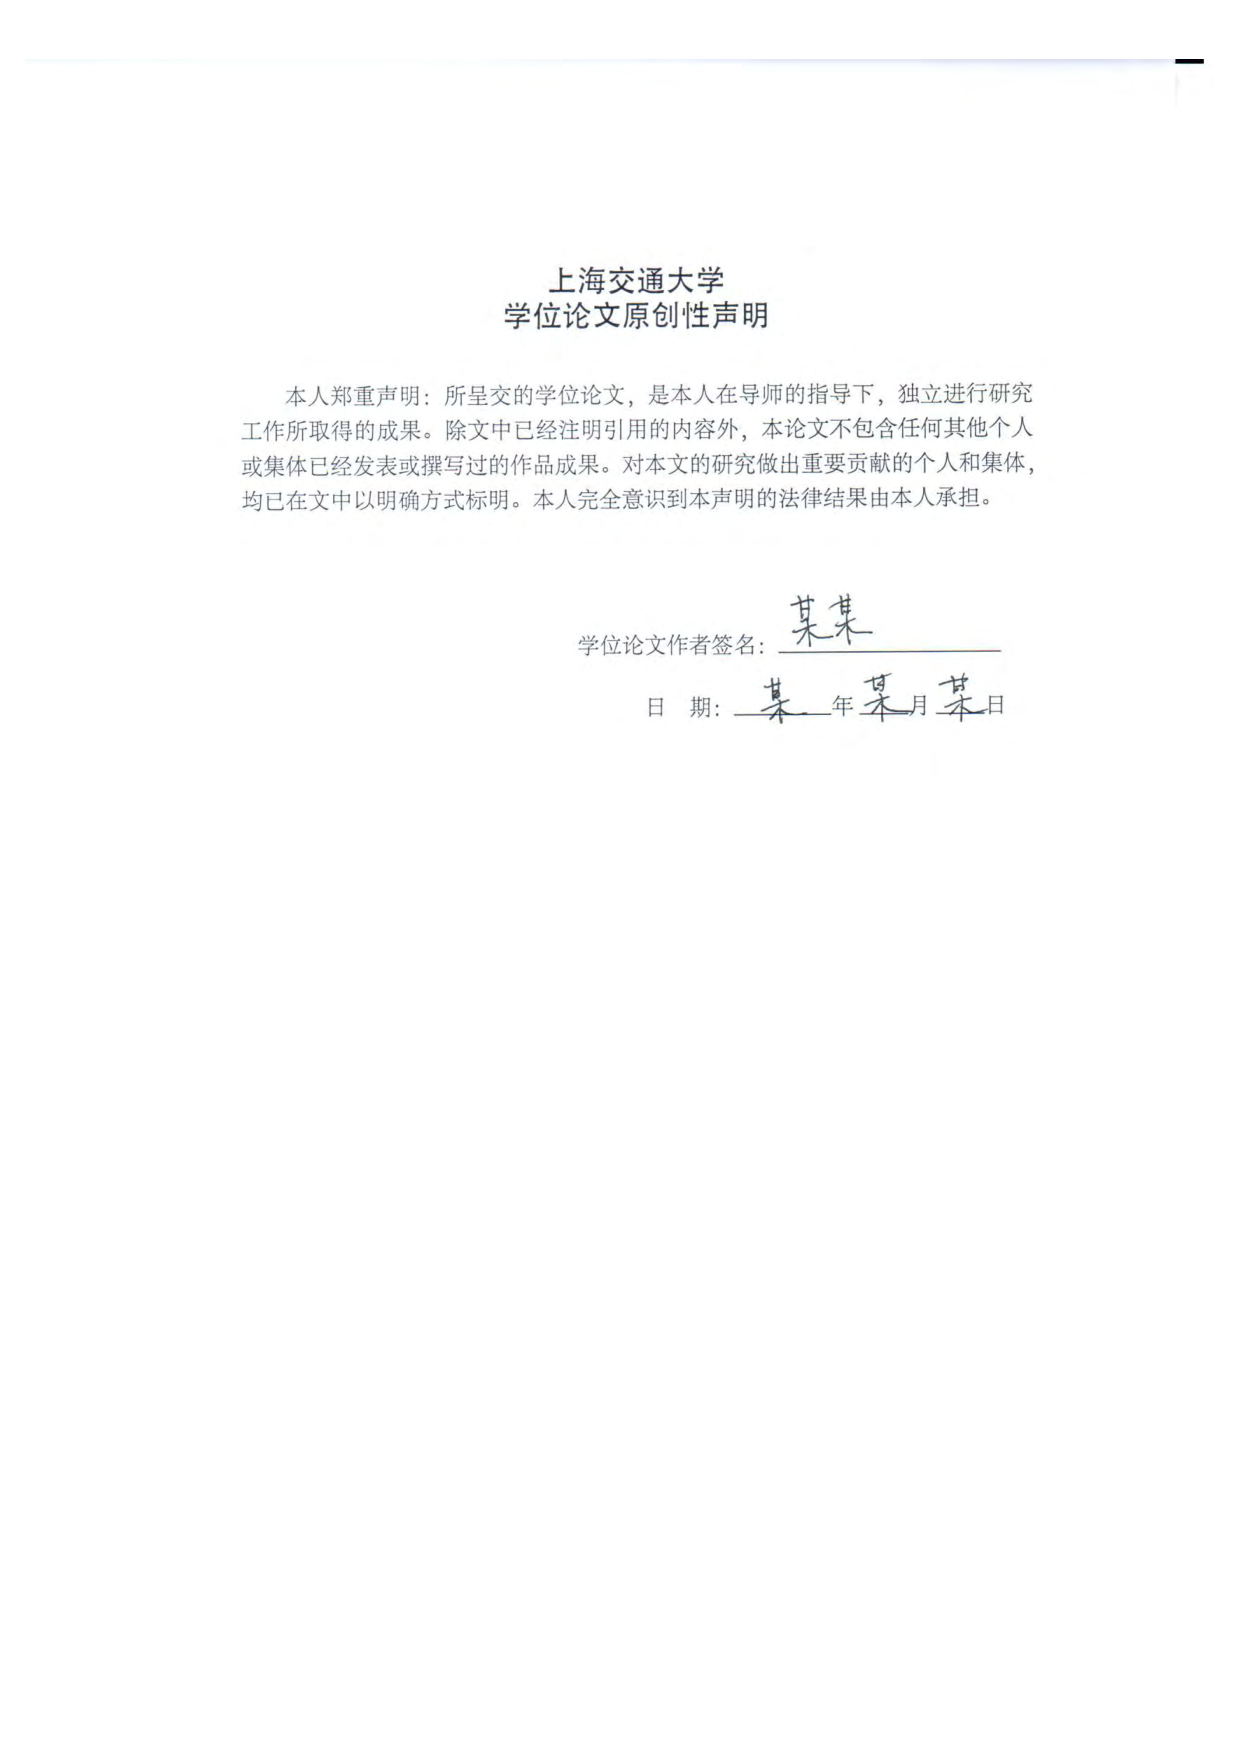
\includepdf{pdf/original.pdf}
	\cleardoublepage
	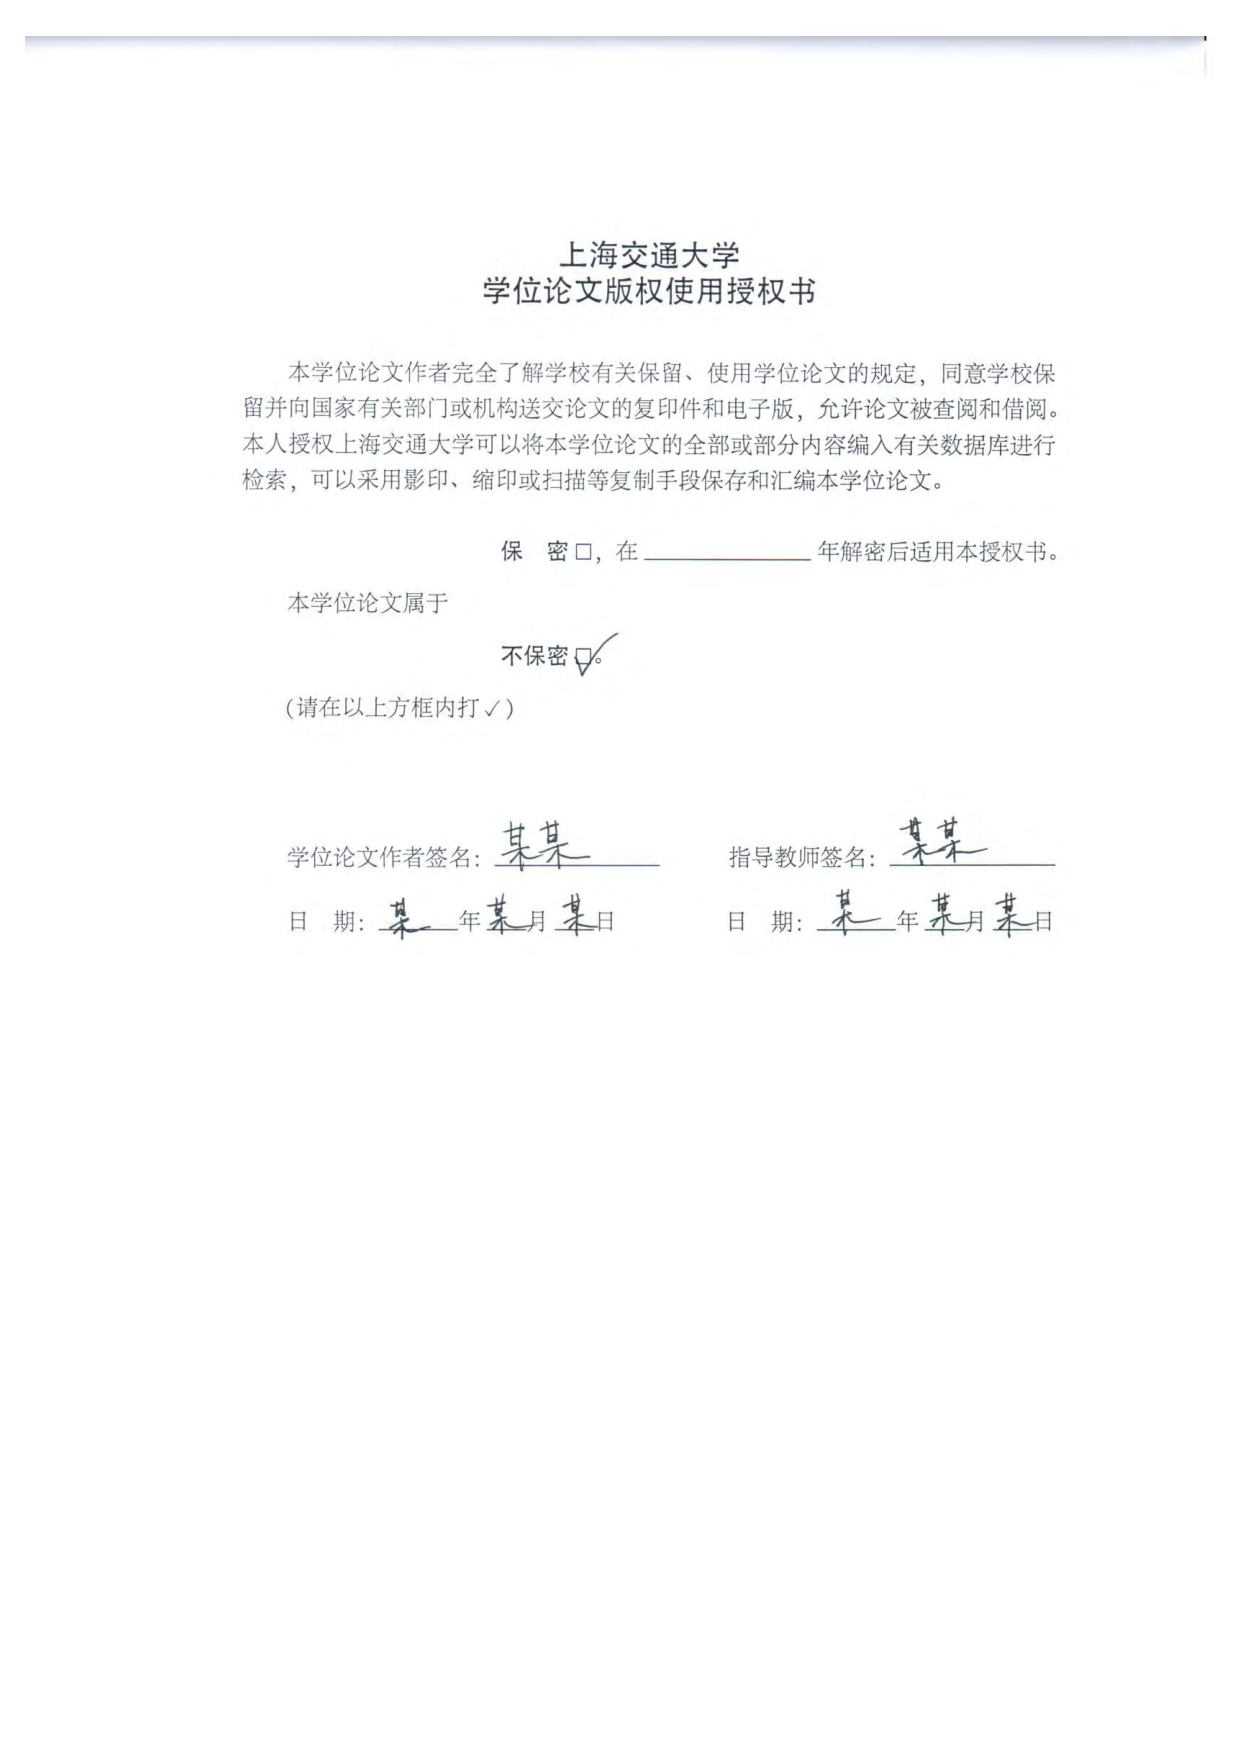
\includepdf{pdf/authorization.pdf}
	\cleardoublepage
\else
	%\makeDeclareOriginal
	%\makeDeclareAuthorization
\fi
\makeatother

\frontmatter    % 使用罗马数字对前言编号

%% 摘要
\pagestyle{main}
%%==================================================
%% abstract.tex for SJTU Master Thesis
%%==================================================

\begin{abstract}
安全数位卡,即SD卡(Secure Digital Memory Card),是一种存储卡,被广泛应用于便携设备上。

单片机,即单片微型计算机(Single-chip Microcomputer),是把中央处理器、存储器、定时/计数器、
各种输入输出接口等都集成在一块集成电路芯片上的微型计算机。
与应用在个人电脑中的通用型微处理器相比,它更强调自供应(不用外接硬件)和节约成本。
它的最大优点是体积小,可放在仪表内部,但存储量小,输入输出接口简单,故需要外接存储设备,SD卡就是经济高效的最佳选择。

然而51单片机并没有SD卡接口,同时,单片机从SD卡读写的数据要与计算机实现兼容性,要求其必须支持相应的文件系统。
鉴于目前计算机大多使用微软(Microsoft)的FAT32文件系统,本课题所要设计的文件接口将在支持FAT32文件系统的同时,
解决51单片机与计算机通过SD卡的通信问题。

本课题通过模块化的设计方法,自顶向下分层设计相应的子模块以实现相应部分功能。并且,
在各个模块之间仅留出下层对上层的函数接口,这样既利于子模块单独测试,又便于各个模块的移植,
同时整个工程框架清晰,层次分明,便于调试。
具体函数的设计实现,各个参数的选取设置均以官方说明文档为准。

为了令本文件接口具有良好的可移植性以及标准性,本课题在设计研究过程中参考了一些开源项目以及官方文档,
严格做到契合相关协议和规范,同时不失自己的特色,为本地差异化配置留出了足够空间。
最终,本接口实现了对FAT32文件系统的挂载识别,文件的打开关闭,创建删除以及读写功能。
对底层的SD卡具有识别能力,能够识别SDSC、SDHC/XC,能够识别「MBR」和「DBR」扇区。

通过本课题的实践,我不仅对FAT32文件系统有了深刻的认识和了解,并且对SD卡的底层协议规范有了彻底的认知,最终,
基于微处理器的文件接口的实现更是说明了在51单片机这类资源有限的微型计算机上搭建对大型文件系统(如FAT32)的接口支持
是可行的。

\keywords{ 单片机,FAT32,SD卡,文件接口 }
\end{abstract}

\begin{englishabstract}

Secure Digital cards, 
a memory card, is widely used in portable devices.

A variety of input and output interfaces are all integrated on a single integrated circuit chip microcomputers,
which is called Single-chip Microcomputer.
Its biggest advantage is small size, can be placed inside of the instrument.
While its poor amounts of storage, it requires an external storage device that SD card is a cost-effective choice.

However, the C8051 MCU have no SD card interface.
Given the mostly computer using Microsoft OS, whose file system is FAT32.
The file interfaces to be designed for this project will support the FAT32 file system at the same time,
C8051 MCU can communicate and share the data with computer by SD card.

The specific functions and parameters will be ruled by official documents.

In order to make the file interface portable and standard, 
reference is made to some open source projects as well as official documents in my design and implementation process.
Strictly to fit the relevant agreements and norms, without losing its own characteristics,
the interface set aside enough space for local specific configuration.
Ultimately, this interface for FAT32 file system can mount and identify file system, open and close files,
create and delete files, and R/W files.
The bottom sub-module has an identification ability to identify SDSC, SDHC / XC, and also MBR or DBR.

Through the practice of the subject, I have a deep knowledge and understanding of the FAT
file system and SD card. Meanwhile, the problem that  MCU shared information and data hard with PC by SD card
has been solved. It proves that MCU communicate with PC through formatted files is available.

\englishkeywords{SDC, MCU, FAT, file interface}
\end{englishabstract}



%% 目录、插图目录、表格目录
\tableofcontents
%\listoffigures
%\addcontentsline{toc}{chapter}{\listfigurename} %将插图目录加入全文目录
%\listoftables
%\addcontentsline{toc}{chapter}{\listtablename}  %将表格目录加入全文目录
%\listofalgorithms
%\addcontentsline{toc}{chapter}{算法索引}  %算法目录加入全文目录

%%%==================================================
%% symbol.tex for SJTUThesis
%% Encoding: UTF-8
%%==================================================

\chapter{主要符号和缩略语对照表}
\label{chap:symb}

\begin{longtable}{ll}
    FAT & \textit{ File Allocated Table}\\
    SDC & \textit{ Secure Digital Card}\\
    SDSC & \textit{ Standard Capacity SD Memory Card}\\
    SDHC & \textit{ High Capacity SD Memory Card}\\
    SDXC & \textit{ Extended Capacity SD Memory Card}\\
    PLSV & \textit{ Physical Layer Specification Version}\\
    CID & \textit{ Card IDentification number}\\
    RCA & \textit{ Relative Card Address}\\
    DSR & \textit{ Drive Stage Register}\\
    CSD & \textit{ Card Specification Data}\\
    SCR & \textit{ SD Configure Register}\\
    OCR & \textit{ Operation Condition Register}\\
    SSR & \textit{ SD Status Register}\\
    CSR & \textit{ Card Statue Register}\\
    SPI & \textit{ The Serial Peripheral Interface bus}\\
    MISO & \textit{ Master Input/Slave Output}\\
    MOSI & \textit{ Master Output/Slave Input}\\
    CRC & \textit{ Cyclic Redundancy Check}\\
    MCU & \textit{ Single Chip Microcontroller}\\
    BIOS & \textit{ Basic Input/Output System }\\
    BPB & \textit{ BIOS Parameter Block}
\end{longtable}
 % 主要符号、缩略词对照表
\mainmatter	% 使用阿拉伯数字对正文编号

%% 正文内容
\pagestyle{main}
%%==================================================
%% chapter01.tex for NWPU Bachelor Thesis
%%==================================================
\chapter{绪论}
\label{chap:Introduction}
本课题是为解决单片机与个人计算机数据共享困难的问题而提出的。
本工程将为此设计并物理实现一个可行的、与FAT32文件系统相兼容的文件接口,它能够为单片机提供文件系统的部分功能,
实现对文件的管理和操作,对数据的组织和传输,同时,与计算机进行数据共享、文件互动也是其重要功能。
\section{背景}
\label{sec:Background}
绝大多数现在的单片机\supercite{mcu1,mcu2}(MCU)都是基于冯·诺伊曼结构的,这种结构清楚地定义了嵌入式系统所必需的四个基本部分:
一个中央处理器核心,程序存储器(只读存储器或者闪存)、数据存储器(随机存储器)、一个或者更多的定时/计数器,
还有用来与外围设备以及扩展资源进行通信的输入/输出端口——所有这些都被集成在单个集成电路芯片上。

单片机时钟频率通常较同时代的计算机芯片低,但它价格低廉,能够提供充足的程序存储器、丰富的片上接口。
某些架构的单片机生产厂商众多,例如8051系列\supercite{mcu3}、Z80系列。一些现代的微控制器支持一些内建的高级编程语言,
比如BASIC语言、C语言\supercite{mcu4}、C++等。

文件配置表(FAT),是一种由微软发明并拥有部分专利\footnote{专利申请在于文件系统中支持\textbf{长文件名\supercite{lfn1}}的技术,
而不是文件系统核心本身}的文件系统,供MS-DOS使用,也是所有非NT核心的微软窗口使用的文件系统。

相对于其他的文件系统,FAT文件系统\supercite{fatms}由于其使用简单的数据结构,使得文件操作耗时、磁盘空间利用率低等性能差的问题在存在许多小文件的情况下尤为突出\supercite{fat5}。
因为FAT文件系统考虑当时电脑性能有限,所以未被复杂化,这使它成为理想的软盘和存储卡文件系统,也适合用作不同操作系统中的数据交流。
传统的FAT32\supercite{fat4,fat8}文件系统能够兼容大容量存储器,所以仍然是便携式数字设备使用最广泛的文件系统\supercite{fatrv}。
\section{问题}
\label{sec:Issues}
如上所述,出于简化和成本的考虑,单片机往往没有配置SD卡\supercite{sdgp}接口,更不用说应的文件系统接口了,这导致单片机与PC计算机的数据共享变得困难。

一个没有文件系统的机器(单片机)和一个有文件系统的机器(计算机)是无法通过格式化的数据(Formatted Data)沟通的。
在没由相应的文件接口的情况下,单片机向SD卡写入的数据是无法被带有文件系统的计算机正确识别的。因为单片机不知道将数据写入到哪里,
也不知道如何组织数据,这不仅不能够正确地写入数据,还可能损坏原本的文件系统甚至损害磁盘媒介\footnote{比如将数据写入了磁盘的「MBR」扇区或者「DBR」扇区}。

反之,单片机从SD卡中读取数据时也无法正确识别按照特定的文件系统格式存放的数据,此时在单片机看来,SD卡中存储的数据是一些杂乱无章的字节。

\section{目标}
\label{sec:Goals}
通过设计并实现一个通用且兼容的文件系统接口(使用SD卡作为传输介质),将极大地方便单片机\supercite{fat6}与个人计算机的通信和数据交流。

此时本课题将设计一个文件系统\supercite{fatfs}接口,为那些自身不具备文件系统的机器(比如单片机),
将数据按照的特定的文件系统的格式组织管理好,同时提供文件系统的部分简化功能,做到与原生的文件系统完全兼容。

\section{方法}
\label{sec:Solution}
为了尽快完成对FAT32文件系统的设计实现和验证工作,本工程简化了不相关的因素(底层环境),故选择比较容易实现的SPI总线协议\supercite{spi1}作为单片机与SD通信\supercite{sdfat1,sdfat2}的方式,
即在SD卡的SPI模式下进行数据的物理传输。同时,微处理器选择了自带SPI硬件接口的C8051F020芯片,使之与一个11脚的SD卡槽相连接,实验平台就搭建完成了。

本文件接口实行模块化设计思路,将整个工程分为两层,各层相对独立,并且上层模块只能通过预留的API接口调用底层模块,底层模块不能主动与上层模块通信。

\section{意义}
\label{sec:Contributions}
FAT32文件系统接口的实现,使得单片机与个人计算机的数据共享变得可能,使得二者间的信息交流与通信方式更加多样化,同时,
通过使用便携式数字存储介质(比如SD卡、闪存盘、移动硬盘等),单片机可以向普通计算机一样,直观方便地组织和管理数据。

本文件接口能够实现的功能为:
\begin{itemize}[noitemsep,topsep=0pt,parsep=0pt,partopsep=0pt,leftmargin=5cm]
    \item SD卡的插入与拔出检测
    \item SDSC/SDHC/SDXC的识别
    \item 磁盘「MBR」扇区的识别
    \item 磁盘「DBR」扇区的定位
    \item FAT文件系统的识别与挂载
    \item 文件的创建与打开
    \item 文件的读出与写入
    \item 在文件的指定位置读写
    \item 文件的删除与关闭
\end{itemize}


\section{组织}
\label{sec:Orgnization}
本文由以下章节组成:
\begin{itemize}
    \item 第\ref{chap:Introduction}章,绪论,主要介绍了本课题的研究背景意义同时简单叙述了研究的整体思路与构想。
    \item 第\ref{chap:Design}章,设计,具体描述了FAT32文件系统接口的构造方式和设计思路。
    \item 第\ref{chap:Implementation}章,实现,具体描述了FAT32文件系统接口的物理实现过程,详细描述了具体函数的构造过程。
    \item 第\ref{chap:Results}章,实验与结果,简要描述了底层模块的实现与相应的实验验证环境,具体描述了本文件接口在具体实验中的验证和应用。
    \item 第\ref{chap:Summary}章,全文总结,对全文做以总结性的阐述。
\end{itemize}

%%==================================================
%% chapter02.tex for NWPU Bachelor Thesis
%% Encoding: UTF-8
%%==================================================

\chapter{设计}
\label{chap:Design}
本章将具体描述FAT32文件系统接口的整体架构和设计思路。
从要求实现的功能出发,将本接口分为两个模块,并为每个模块都设计符合规定的应用程序接口(API)以供上层程序调用。
本章仅在逻辑层面进行工程的设计描述,具体的算法实现将在第\ref{chap:Implementation}章详述。

\section{架构设计}
\label{sec:Architecture}
通过分层的模块化设计,将整个文件接口要求达成的功能全部通过上层模块的预留API体现出来,这样,顶层的用户应用程序也无需关心底层的驱动和硬件。
分层如下:
\begin{enumerate}[noitemsep,topsep=0pt,parsep=0pt,partopsep=0pt]
    \item
FAT文件系统模块,主要是FAT32文件系统的设计,包括识别并挂载FAT32文件系统、创建并打开文件、在文件中读取数据和写入数据、修改数据等功能,
控制着数据在磁盘卷的具体组织形式,在逻辑上负责了磁盘和内存的数据交互。
    \item
SD卡驱动模块,主要是SD卡相关函数功能的设计,包括SD卡初始化进入SPI模式、读写扇区数据等功能,是联系整个软件层与硬件层的桥梁,控制着数据的物理传输。
\end{enumerate}

\begin{figure}[!htb]
    \centering
    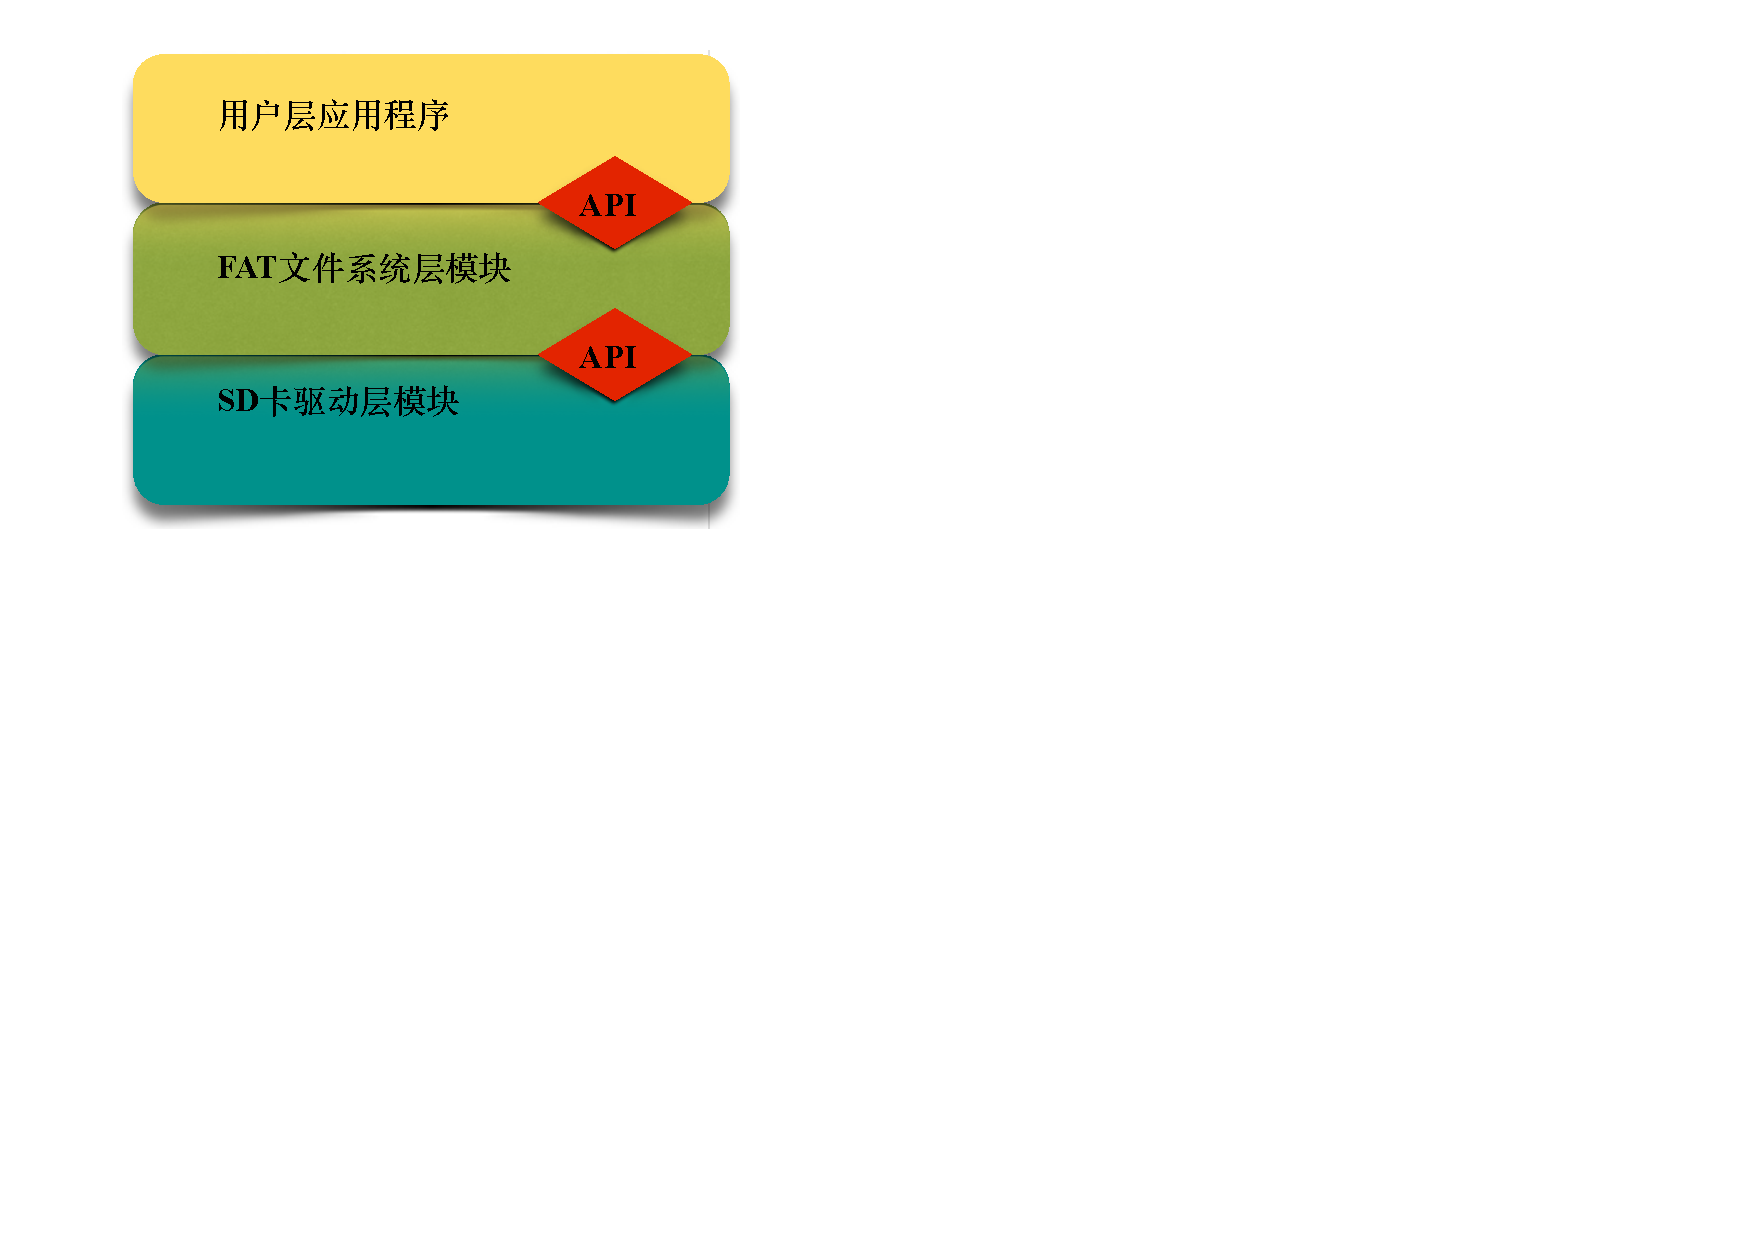
\includegraphics[width=0.5\textwidth]{chap2/layer.pdf}
    \\
    \caption{整体的架构层次}\label{fig:specflow}
\end{figure}

\section{API设计}
\label{sec:API}
通过研究第\ref{sec:Contributions}节的文件系统接口的实际功能和作用,可以完成上层模块的API设计,
该模块的API将为用户的应用程序提供服务,可以被用户程序调用,具体接口如下:
\begin{longtable}[!htb]{ll}
\caption{FAT文件系统模块的API} \label{tab:fatapi}\\
    \toprule
    f\_detect() & SD卡插入检测 \\ \midrule
    f\_mount() & FAT文件系统的挂载\\ \midrule
    f\_open() & 创建新文件或打开文件\\ \midrule
    f\_close() & 关闭文件\\ \midrule
    f\_read() & 从文件读出指定大小的数据到缓存\\ \midrule
    f\_write() & 从缓存写入指定大小的数据到文件\\ \midrule
    f\_seek\_ptr() & 重设文件中的读写指针位置\\ \midrule
    f\_rm() & 删除文件\\
    \bottomrule
\end{longtable}

考虑到FAT模块需要与底层的硬件层通信,本工程在相应的SD卡驱动模块上也留出了API接口,以供FAT模块调用,
FAT模块通过驱动模块实现了数据的物理传输。
\begin{longtable}[!htb]{ll}
\caption{SD卡驱动模块的API} \label{tab:sdapi}\\
    \toprule
    disk\_initialize () & 底层硬件设备的初始化\\ \midrule
    disk\_read () & 读扇区块(512字节)\\ \midrule
    disk\_write () & 写扇区块(512字节)\\ \midrule
    disk\_offset() & 修正逻辑扇区号与物理扇区号的偏移\\
    \bottomrule
\end{longtable}

\section{FAT32文件系统设计}
\label{sec:FAT32}
整个FAT文件系统最初是基于IBM的PC架构而研发的,由此有一个很重要的特性就是,
FAT文件系统在磁盘上的数据是以小端模式\footnote{与此相对的,还存在另一种存储方式,
即大端模式(Big Endian)}(Little Endian)存储的。
\begin{table}[!htb]
  \centering
  \caption[小端模式存储示例]{32位数据在小端模式下的结构}\label{tab:littleendian}
  \begin{tabular}{lcr} \toprule
      byte[3] & &3 3 2 2 2 2 2 2 \\
              & &1 0 9 8 7 6 5 4 \\
      byte[2] & &2 2 2 2 1 1 1 1 \\
              & &3 2 1 0 9 8 7 6 \\
      byte[1] & &1 1 1 1 1 1 0 0 \\
              & &5 4 3 2 1 0 9 8 \\
      byte[0] & &0 0 0 0 0 0 0 0 \\
              & &7 6 5 4 3 2 1 0 \\ \bottomrule
  \end{tabular}
\end{table}

\noindent 一个FAT文件系统卷由四个基本区域组成,它们顺序排列如下:
\begin{enumerate}[noitemsep,topsep=0pt,parsep=0pt,partopsep=0pt,leftmargin=1cm]
    \item[0) ––]
保留区(Reserved Region),磁盘卷上第一个重要的数据结构被称作BPB(BIOS Parameter Block),它位于保留区域(Reserved Region)的第一个扇区。该扇区有时又被称为启动扇区(Boot Sector)或零号扇区($0^{th}$ Sector)。
    \item[1) ––]
FAT表区(FAT Region),文件分配表,是由一些32比特大小的记录项组成的表,它所占据的扇区数目同样在BPB结构用定义,具体位置是「36」字节偏移位置。FAT32通常有FAT数据结构的两份拷贝,这是出于冗余性的考虑。
    \item[2) ––]
根目录区\footnote{FAT32文件系统卷不存在根目录区,相对应地它存在一个动态的根目录表}(Root Directory Region),通常都是将根目录区放在本区域的第一个簇。簇「Cluster」,是由固定数目组成的相邻扇区集群,这个数目在BPB中定义,处于启动扇区的「13」字节偏移位。
    \item[3) ––]
数据区(File and Directory Data Region),包含了磁盘卷剩余的所有扇区,是文件和目录数据真正存储的地方。
\end{enumerate}

FAT表是一张记录了哪些簇号已用、空闲或不可用的表,不仅如此,它还记录了文件的簇链信息。鉴于所使用的FAT文件系统类型不同和磁盘卷的大小不一,一个簇包含的扇区数目可以有多种取值,具体值可以在「BPB」中进行定义。
对于FAT32,尽管FAT表的一条记录项有32位的长度,但只有低28位可用,因此FAT32文件系统可以支援的最大磁盘卷容量是$2^{28} \times 64 \times 512$字节\footnote{此处的「64」为每簇扇区数的最大可用值,「512」为扇区字节数的推荐值},即8TB。

FAT32卷上的每一个文件或目录(根目录除外)都在父目录表上有一条记录,包含着『名称』、『属性』、『大小』以及32位长度的『起始簇号』等信息。
FAT文件系统中的目录,在物理上与文件有相同的组织形式,这种特殊的文件是由一系列32字节的目录记录(Directory Entry)所组成的表,
故目录文件实际上是一张动态的目录表。
FAT32的根目录\footnote{根目录,Root Directory,其起始簇号通常被分配为「2」号簇,故往往是在数据区最开始的扇区簇中。}的与普通目录的不同之处在于,根目录没有时间戳(Date or Time Stamps),没有文件名(只有隐含文件名「\textbackslash」),并且没有「当前目录」(「.」)文件和「父目录」(「..」)文件。另外,根目录还有比较特殊的一点是,它是文件卷上唯一一个可以合法拥有「ATTR\_VOLUME\_ID」标志位的文件。

要完成FAT32文件系统模块的设计,首先要将该模块进一步细分。
在之前的API中,「f\_open()」、「f\_rm()」两个函数需要创建和删除文件,这其中涉及到了对FAT表操作,
最主要的就是新建或者续接簇链(「create\_chain()」)和删除簇链(「remove\_chain()」)。在更新簇链时,
需要对FAT表项进行读取(「get\_fat()」)和更新(「put\_fat()」)。
这两个函数还涉及到了对父目录表的操作,如在目录表上注册一条记录项(「dir\_register()」)、在目录表中寻找指定的记录(「dir\_find()」)、
目录表指针回溯(「dir\_rewind()」)以及指针指向下一条目录项(「dir\_next()」)等。

对「f\_read()」和「f\_write()」函数,如果读写的字节不跨簇的话,不需要与FAT表交互。否则,同样需要通过访问FAT表,遍历文件所在的簇链进行读写。
特别地是,读函数不需要更新FAT表的记录,而写函数有可能会调用「create\_chain()」函数,因为当写入的字节超过已分配的空间时需要向FAT表申请更多的簇来储存数据。

「f\_mount()」函数只需要调用驱动层的初始化函数,之后正确识别并载入「DBR」的启动扇区到内存,最后读取相应的参数信息并使标志位有效即可完成挂载操作。
现在直观地描述如下:

\begin{lstlisting}[basicstyle=\small\ttfamily,caption={FAT文件系统模块结构},label=layout,numbers=none]
├─── f_mount()
├─── f_detect()
├─── f_open()
│       ├────── dir_register()
│       │           ├──────── dir_next()
│       │           ├──────── create_chain()
│       │           │               ├─────── get_fat()
│       │           │               └─────── put_fat()
│       │           └──────── dir_rewind()
│       └────── dir_find()
├─── f_read()
│       └────── getfat()
├─── f_write()
│       ├────── getfat()
│       └────── create_chain()
│                ├──────── get_fat()
│                └──────── put_fat()
├─── f_rm()
│       ├────── dir_find()
│       ├────── get_cluster()
│       └────── remove_chain()
│                ├──────── get_fat()
│                └──────── put_fat()
├─── f_seek_ptr()
└─── f_close()
\end{lstlisting}

上图中的每一次缩进,都表示函数进行了一次调用,对驱动层函数(disk\_read()等)的调用没有画出来。
「f\_detect()」、「f\_close()」等函数相对比较容易实现,对于「f\_open()」、「f\_write()」而言相对复杂一些,
这些函数的具体实现方法将留在\ref{chap:Implementation}详述。

\section{硬件驱动模块的设计}
\label{sec:Driver}
如前所述,SD卡的驱动模块选择了SPI总线协议完成单片机与SD卡的通信,
故在本模块主要需要实现的是由内存向硬件(在本实验中是SD卡)中写入数据以及从中读取数据到内存,
分别由「disk\_read()」和「disk\_write()」实现。鉴于扇区字节数通常都是512字节,并且单片机的内存也是紧俏资源,
故使每次读写的数据块大小都为512字节,即一个扇区。

对于多数磁盘卷,「DBR」扇区往往不是物理扇区第一块,而是由于隐藏扇区的关系有一个偏移值,「disk\_offset()」会完成逻辑扇区号与物理扇区号之间的转换。

\section{小结}
\label{sec:Sum2}
本章具体描述了本工程的整体架构以及各模块预留的应用程序接口,简要剖析了FAT文件系统的设计思路,
描述了FAT模块相关函数的作用功能以及各自的相互调用关系,勾勒出了FAT文件系统模块的大体轮廓,
同时,简要描述了SD卡驱动模块的主要函数和功能,为之后的具体实现做好了理论准备。

%%==================================================
%% chapter04.tex for NWPU Bachelor Thesis
%% Encoding: UTF-8
%%==================================================

\chapter{实现}
\label{chap:Implementation}
之前的章节阐述了文件系统接口的逻辑设计,本章将继续描述文件接口的具体实现方法。
对于上层的FAT文件系统模块,主要负责在逻辑上完成需求的各项功能,是文件接口的核心。
该模块与具体硬件层无关,故具有良好的可移植性和拓展性。然而要实现一个文件系统接口并进行实验验证,硬件层必不可少,
而SD卡的驱动模块就负责联系文件系统模块与硬件层,控制数据的物理传输。

\section{预定义}
\label{sec:Defination}
鉴于「int」类型在不同CPU\footnote{32位CPU和64位CPU的「int」长度不一,并且,不同编译器也可能出现对「int」的不同定义。}上有不同的定义长度,
为了尽可能满足可移植性的要求,本工程仅使用以下三种固定长度的数据类型,
同时,为了使用方便,本工程将不同长度的数据类型分别重新定义为「BYTE」、「WORD」和「DWORD」:
\begin{lstlisting}[language={C}, caption={数据类型重定义}]
//长8位
typedef unsigned char	BYTE;
//长16位
typedef unsigned short	WORD;
//长32位
typedef unsigned long	DWORD;
\end{lstlisting}

接下来可以定义所需的结构体了。由于本工程不是很复杂,所以文件系统(FatFS)的结构体中除了包含FAT32文件系统参数信息之外,
还包含了文件的信息(比如文件指针、文件大小、起始簇号等)。
\begin{lstlisting}[language={C}, caption={文件系统数据类型}]
typedef struct {
	BYTE	fs_type;        //FAT文件系统的类型(FAT12、FAT16或FAT32)
	BYTE	csize;          //簇大小(单位为扇区)
	DWORD	n_fatent;       //FAT表的总记录数(卷可用簇数加2)
    DWORD   fatsize;        //单张FAT表的大小
	DWORD	fatbase;        //首张FAT表的起始地址(单位为扇区)
	DWORD	dirbase;        //根目录区起始地址(单位为扇区)
	DWORD	database;       //数据区起始地址(单位为扇区)
    //FSINFO项
    WORD    fsi_sec;        //FSINFO 的扇区号
    DWORD   freecont;       //空闲簇数
    DWORD   nxtfree;        //下个空闲簇号
    // 文件项
    BYTE    flag;           //文件的标志位(判断打开关闭)
    DWORD	fptr;           //文件的读写指针
	DWORD	fsize;          //文件大小
	DWORD	org_clust;      //文件起始簇号
	DWORD	curr_clust;     //文件当前簇号
	DWORD	curr_sect;		//文件当前扇区号
} FATFS;
\end{lstlisting}
除此外,还定义了目录项(Directory Entry)的结构体。
\begin{lstlisting}[language={C}, caption={目录项数据类型}]
typedef struct {
	WORD	index;          //该目录项在目录表的序号
	BYTE	fn[12];         //文件名
	DWORD	sclust;         //目录表的起始簇号
	DWORD	clust;          //目录表的当前簇号
	DWORD	sect;           //目录表的当前扇区号
} DIR;
\end{lstlisting}

\section{文件系统相关函数的实现}
\label{sec:Function}
对于FAT文件系统模块,需要始终维护一个FATFS类型的全局变量的指针$fs$,$fs$指向的变量将记录并及时更新文件系统的信息。
\subsection{挂载文件系统}
\label{sec:Mount}
在文件接口要求的所有功能中,挂载文件系统总是第一步\footnote{SD的插拔检测过于容易,本章暂且按下不表,下章会再次说明。}要做的,
其他的后续操作只有在文件系统成功挂载的情况下才变得可行。
而挂载文件系统的第一步,是能够正确无误\footnote{此处的正确无误指在逻辑上无错误,至于物理上的传输无误由底层的驱动模块保证。}的读入「DBR」扇区,
因为多数磁盘的「MBR」扇区才是物理上的$0^{th}$扇区,在「MBR」与「DBR」之间存在一定数目的隐藏扇区。因此,首要任务是分辨「MBR」和「DBR」,
同时正确定位「DBR」的位置。本模块不需对扇区进行逐块比较,而是采用一种更加快捷的办法:
\begin{balgo}{定位「DBR」扇区}{algo:dbr}
\begin{algorithmic}
\Require buff[512]\Comment{内存开辟一块缓冲池,单位字节,用来暂存从磁盘读出的数据}
\If{WORD(buff $+$510) $\neq$  0xAA55 }\Comment{是否是启动扇区}
    \State \Return Error: Not Boot Sector
\ElsIf{buff[0] $\neq$ (0xEB $and$ 0xE9)} \Comment{「DBR」的首字节必须是0xEB或0xE9}
    \State \Return DWORD(buff $+$454)\Comment{从0x1C6(454)开始的4个字节是「DBR」扇区号}
\EndIf
\end{algorithmic}
\end{balgo}

其中,「WORD(addr)」和「DWORD(addr)」分别指采用大端模式从$addr$读出16位数(字)和32位数(双字)。
通过算法\ref{algo:dbr}就可以取得正确的「DBR」扇区号了,之后要做的就是读入启动扇区(Boot Sector),
并更新$*fs$的各项信息。而且,由于使用的文件系统是FAT32,还要在读入逻辑上的$1^{st}$扇区,这个扇区记录了FSINFO的相关信息,
同样需要在$*fs$中进行更新,具体判断和定位「DBR」扇区的方法以及挂载文件系统的流程可见图\ref{fig:fsmount}。
\begin{figure}[!htb]
    \centering
    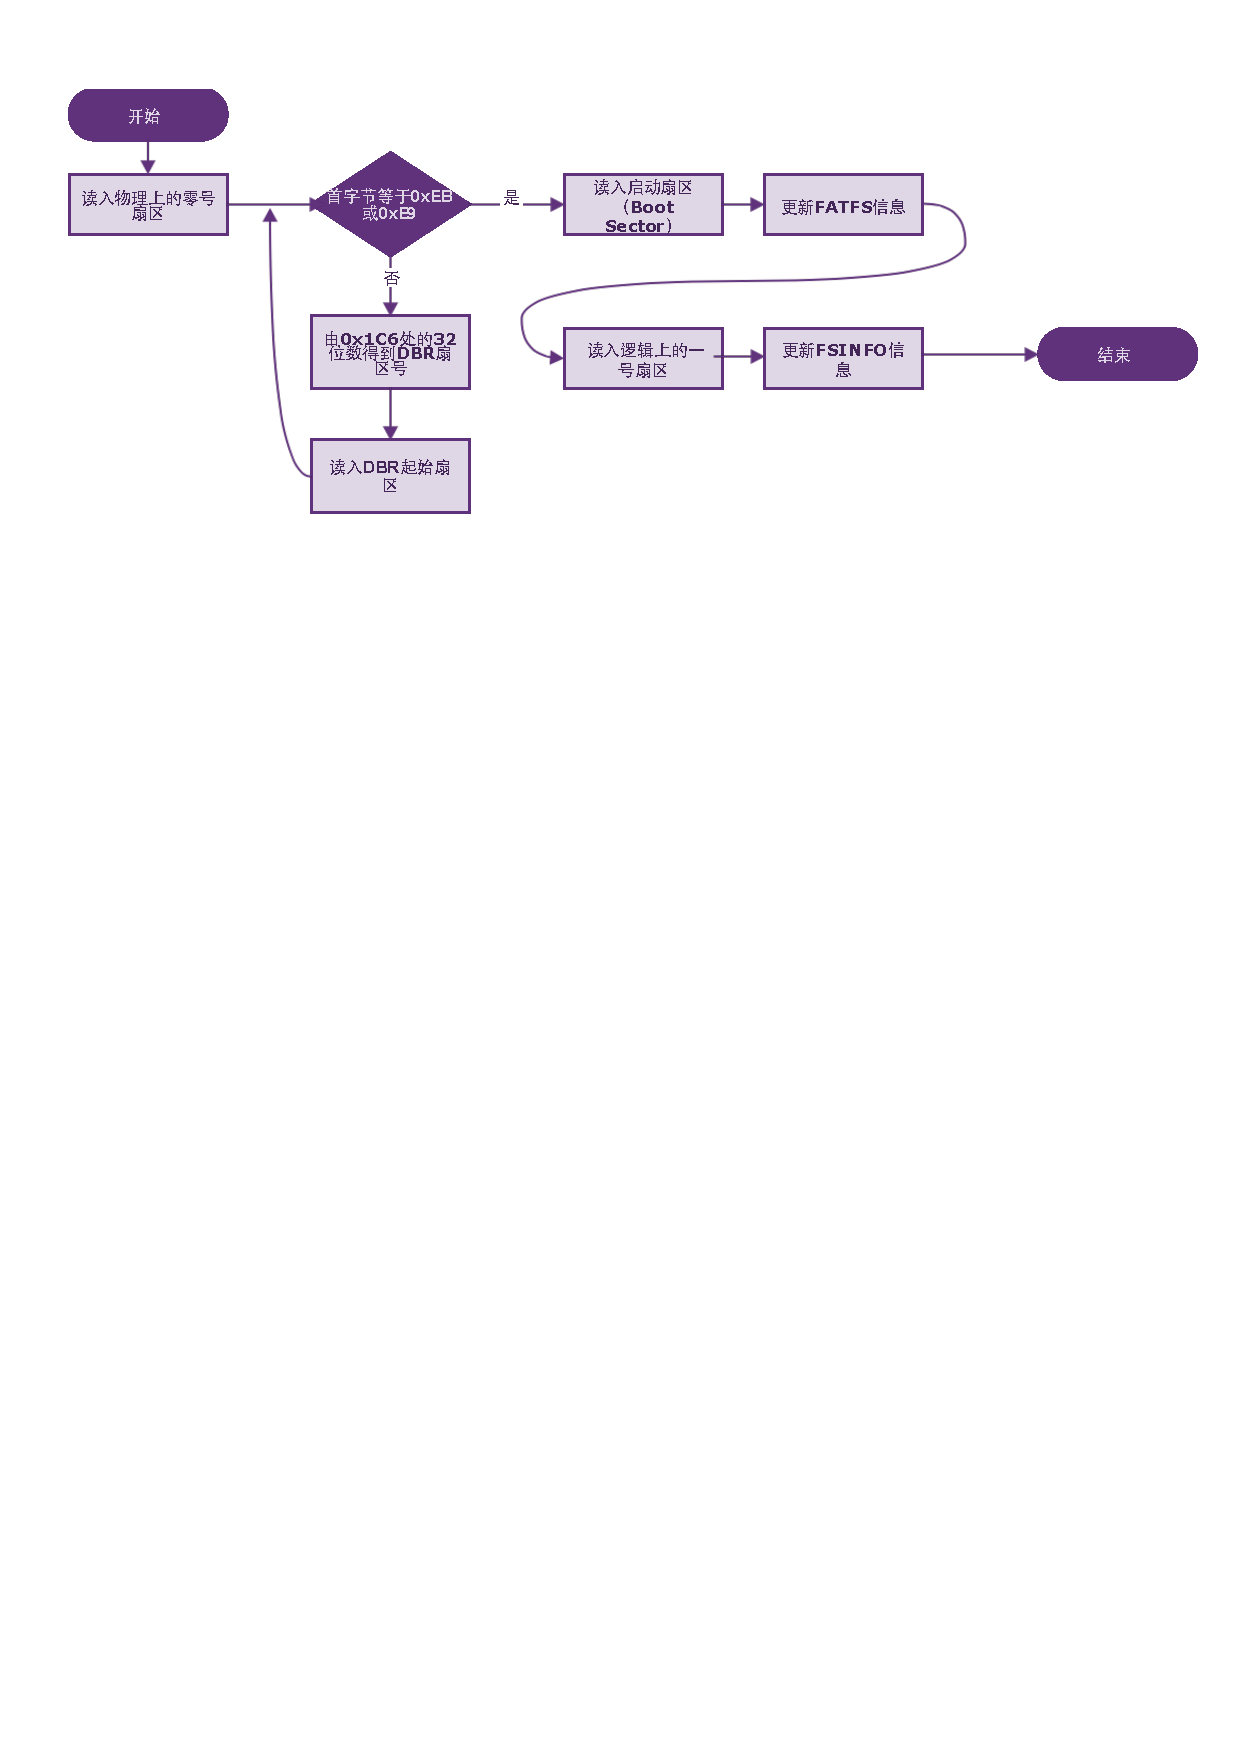
\includegraphics[width=1.0\textwidth]{chap3/mount.pdf}
    \\
    \caption{挂载文件系统}\label{fig:fsmount}
\end{figure}

\subsection{文件的创建与删除}
\label{sec:Create}
创建删除文件是相对而言比较复杂的操作,因为它们不仅设计的对FAT表的操作,还涉及到了对目录表的操作。
文件的创建或删除,要先在父目录中查找文件,对于创建操作,若查找返回无文件则可以新建文件,包含了在父目录表中登记目录项记录和在FAT表中新建簇链两个操作;
对于文件的删除操作,若查找成功则可以删除文件,包含了在父目录表中删除目录项记录和在FAT表中删除簇链。
具体的判断流程见图\ref{fig:crtdel}。
\begin{figure}[!htb]
    \centering
    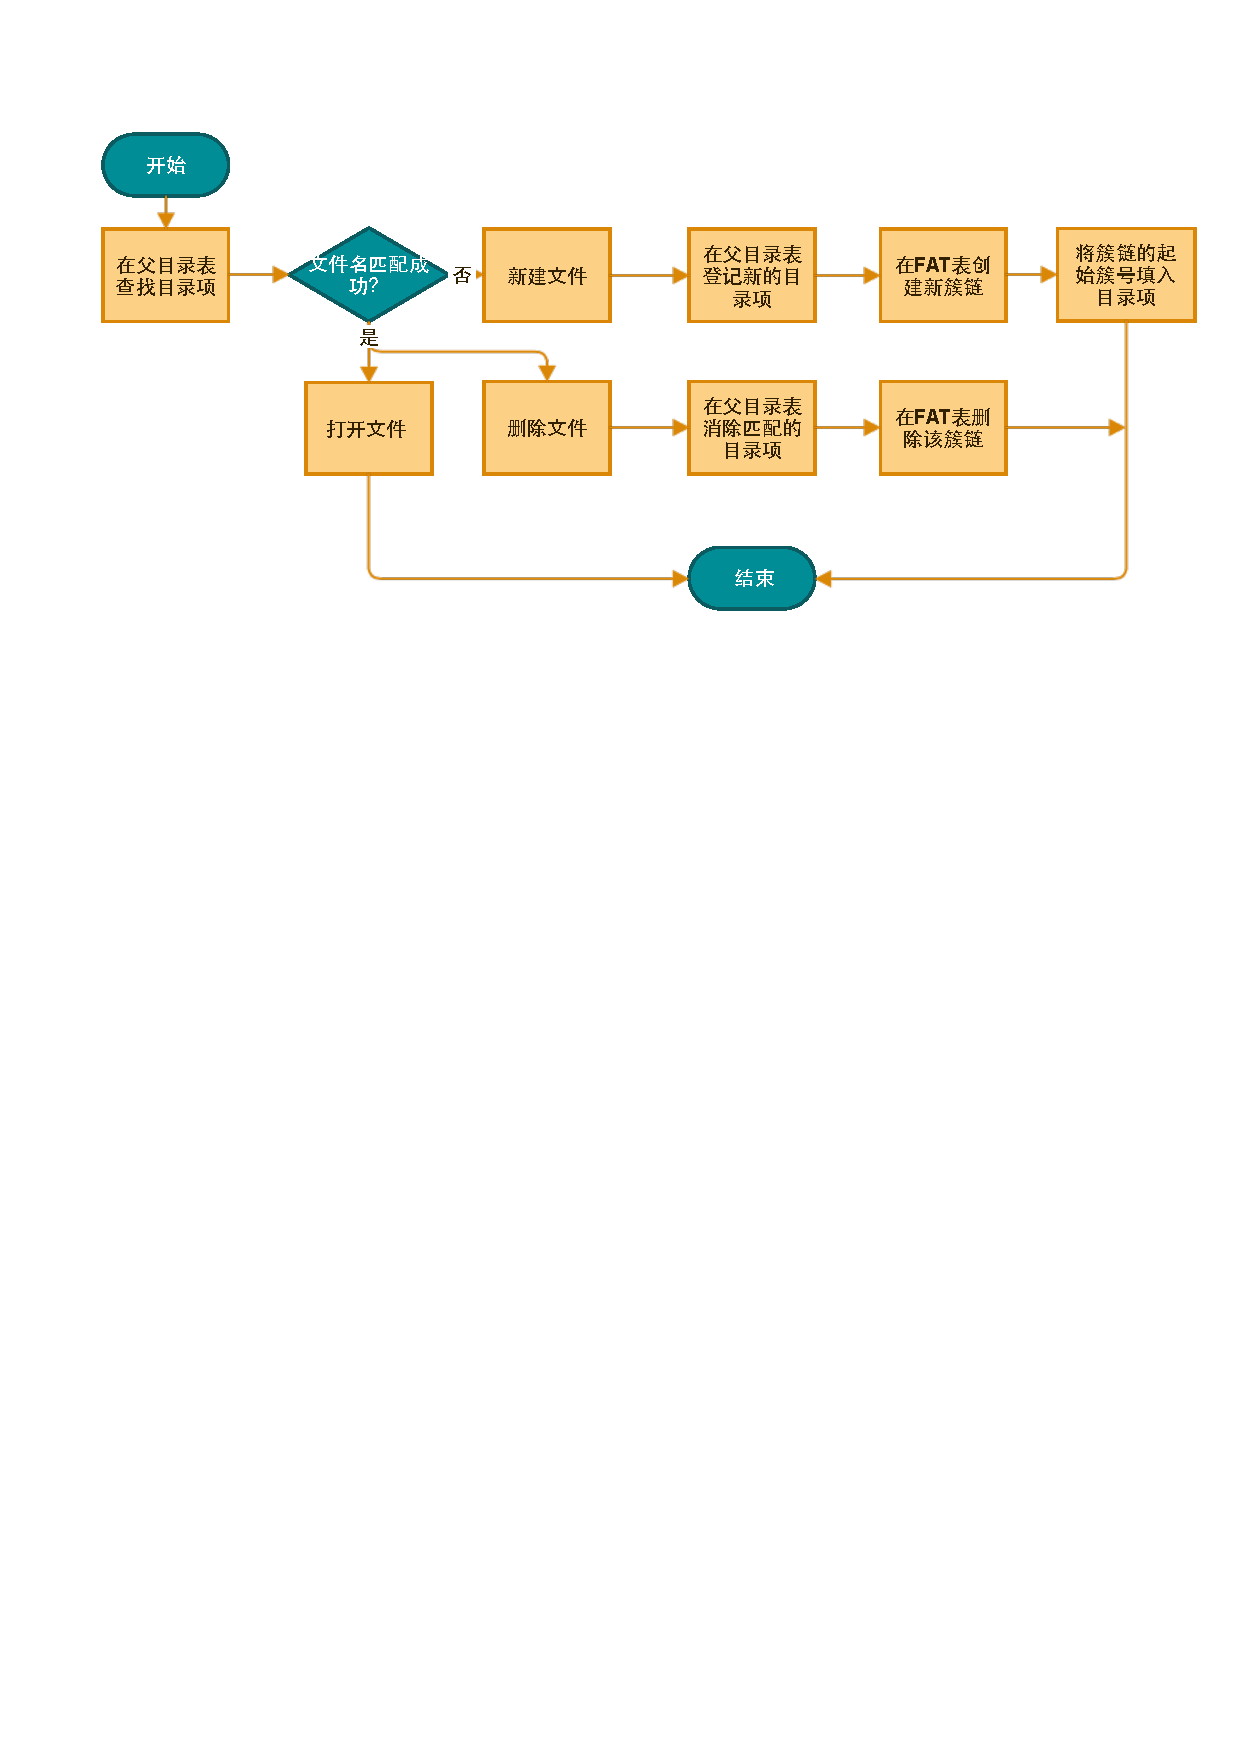
\includegraphics[width=1.0\textwidth]{chap3/creatdel.pdf}
    \\
    \caption{创建或删除文件}\label{fig:crtdel}
\end{figure}
\subsubsection{目录操作}
\label{sec:dir}
首先,实现对目录表的操作,即在一张目录表(本工程中,始终是在根目录操作)中登记(Register)一条32字节大小的目录项或者删除一条记录。
无论是登记还是删除,都需要先在该目录表上进行查找,查找是采用文件名匹配的方式,当找一个空闲的可用目录项时,结束查找。

在查找目录项的过程中,要用到两个操作「Rewind」和「Next」。顾名思义,「Rewind」就是将目录表上的指针复位,使其回到目录表的起始目录项处,
「Next」就是将指针前进32字节,即将指针指向下一个目录项。由于FAT32文件系统的规定,扇区字节数必须能够被「512」整除,且每簇扇区数都是2的整数次幂,
因此目录项总能够与扇区或者簇的边界对齐,任一条目录项都不会横跨两个扇区。
\begin{balgo}{指针越界判断}{algo:boundry}
\begin{algorithmic}
\Require Index \Comment{目录项在目录表中的序号,从$0$开始}
\If{Index $\bmod{(\frac{512}{32})} = 0$}\Comment{到达扇区边界?}
    \If{Index $\div ( \frac{512}{32} )=$ fs->csize} \Comment{到达簇边界?}
    \State Need to change the cluster
    \Else\Comment{不需换簇}
    \State Need to switch to next sector
    \EndIf
\Else\Comment{尚在同一扇区}
    \State No exceeding
\EndIf
\end{algorithmic}
\end{balgo}
因此通过算法\ref{algo:boundry}可以判断指针是否以及到达扇区或簇的边界,若只是到达扇区边界,只需从磁盘读入相邻的下一扇区,覆盖掉当前内存缓冲池「buff」即可。
但如果是到达簇边界,则需要进入FAT表的相应簇号记录项处,沿着簇链取得下一簇号,具体情况在第\ref{sec:fat}节描述。

在查找目录项时,采用文件名匹配方式,即将文件名当做一个字符串进行匹配。在FAT32文件系统的规范中,短文件名「SFN」的格式必须是「8+3」,即文件名长8字节,
扩展名长3字节,并且鉴于FAT文件系统对字母大小写不敏感,因此存入目录项中的文件名一律都是大写字母。
这样一来,通过<string.h>提供的「memcmp」函数就可以很容易地实现文件名匹配操作。
但是,对空闲目录项的判别并不是文件名匹配,而是判断该目录项的第一个字节是否为「0xE5」或「0x00」。
如果指针指向的目录项首字节为「0xE5」,表明该目录项空闲可用;如果是「0x00」,则表明之后的包含此目录项在内的所有目录项都空闲可用。

一旦找到一条可用的空闲目录项,对于登记目录项操作,此时需要将准备好的『文件名』写入32字节目录项前11个字节,紧跟的字节一般都会填入「0x20」,
即表明该目录项是普通文档而非目录。至于『时间戳』,可以不填写,默认置零即可。『文件大小』在新登记的目录项中是零,之后可能会根据写入的数据大小而更改。
最重要的部分是目录项的『起始簇号』,这个32位的簇号会分为高16位和低16位分别填入,至于簇号怎样得到,具体参见\ref{sec:fat}。
至于删除记录项,仅需将首字节置为「0xE5」,同时要取得相应的『起始簇号』,具体参见\ref{sec:fat}。

\subsubsection{FAT操作}
\label{sec:fat}
如前所述,对于文件创建操作,当在目录表中登记了一条新记录后,只需再进入FAT表新建一个簇链并将相应簇号录入该目录项即完成了文件的创建操作。
至于文件的删除,当在目录表中删除了一条记录同时取得其起始簇号后,还要进入FAT表删除相应的簇链。

因此,现在将问题转变成了新建簇链和删除簇链。
新建簇链要先查找一个可用的空闲簇号,
这里会用到FAT32文件系统所特有的数据结构FSINFO,通过其记录的「fs->nxtfree」,指明了当前FAT表最后一个分配的簇号。
查找空闲簇号时只需从「fs->nxtfree」处开始遍历整张FAT即可,如果该值为「0xFFFFFFFF」表明此值无效,此时要从「2」号簇开始遍历。
一旦找到一个空闲簇号,在其处写入「0x0FFFFFFF」\footnote{「EOC」标记}即表示该簇已被占用,且是当前簇链的最后一个簇号,然后将该簇号返回即可,
对于创建文件操作,这个簇号就是其目录项的『起始簇号』,也是这个文件数据存储的起始簇号。

至于删除簇链,进入FAT表并直接定位到给定的簇号处,接着开始遍历以这个簇号起始的簇链,遍历的同时删除每一个遍历到的簇号
(删除簇号就是将「0x00000000」作为值写入),直到这条簇链遍历结束。至此,簇链的删除就完成了。

在对FAT操作的过程中,只能操作低28位,高4位不可变更。即写入FAT表记录项的值时,要保留其高四位(通过『或』操作和『与』操作完成),
而读出值时要忽略高四位,一般将其清零即可。

\subsection{文件的打开与关闭}
\label{sec:Open}
文件的打开操作实际已经包含在文件的创建操作中,当文件不存在时,文件的打开操作退化为文件的创建操作;当文件已经存在时,
只需读入目录表中的该文件的相关目录项记录的信息,如文件大小、起始簇号等,之后将文件的读写指针清零,同时置文件的标志位有效,即表明文件已打开。

文件的关闭操作相类似,文件不存在时返回错误信息;文件存在时,最主要的是将文件标志位清零,然后将其他信息如读写指针、文件大小等清零即可。

\subsection{文件的读写}
\label{sec:Read}
对文件进行读写数据是本文件接口最主要的功能,并且读写操作互为逆操作,其中向文件中写数据相比读数据要更复杂一些。
读写文件函数需要的参数包括:缓存区地址、未传输字节数和总共要传输的字节数,其中,未传输字节数初始值为零。
读文件内的数据到缓存,首先要求判断文件是否以及打开,具体通过$*fs$中的文件标志位进行判断。

在文件成功打开的情况下,判断尚未传输的字节数是否大于「fs->fsize」与「fs->fptr」的差,如果是,则说明当前文件容量不足以供这么多的字节进行写入或读出,
如果当前操作是读操作,那么提供的要求读出的字节数超限,直接截断,按照文件大小读取数据;
但是,如果当前操作是写操作,当待写字节数超限时,需要更新文件大小「fs->fsize」的值,并且,每当分配的簇空间不足时,要进行续接簇链操作,
以取得更多的簇供数据写入。

具体的读写文件过程如图\ref{fig:freadflow}所示。
\begin{figure}[!htbp]
    \centering
    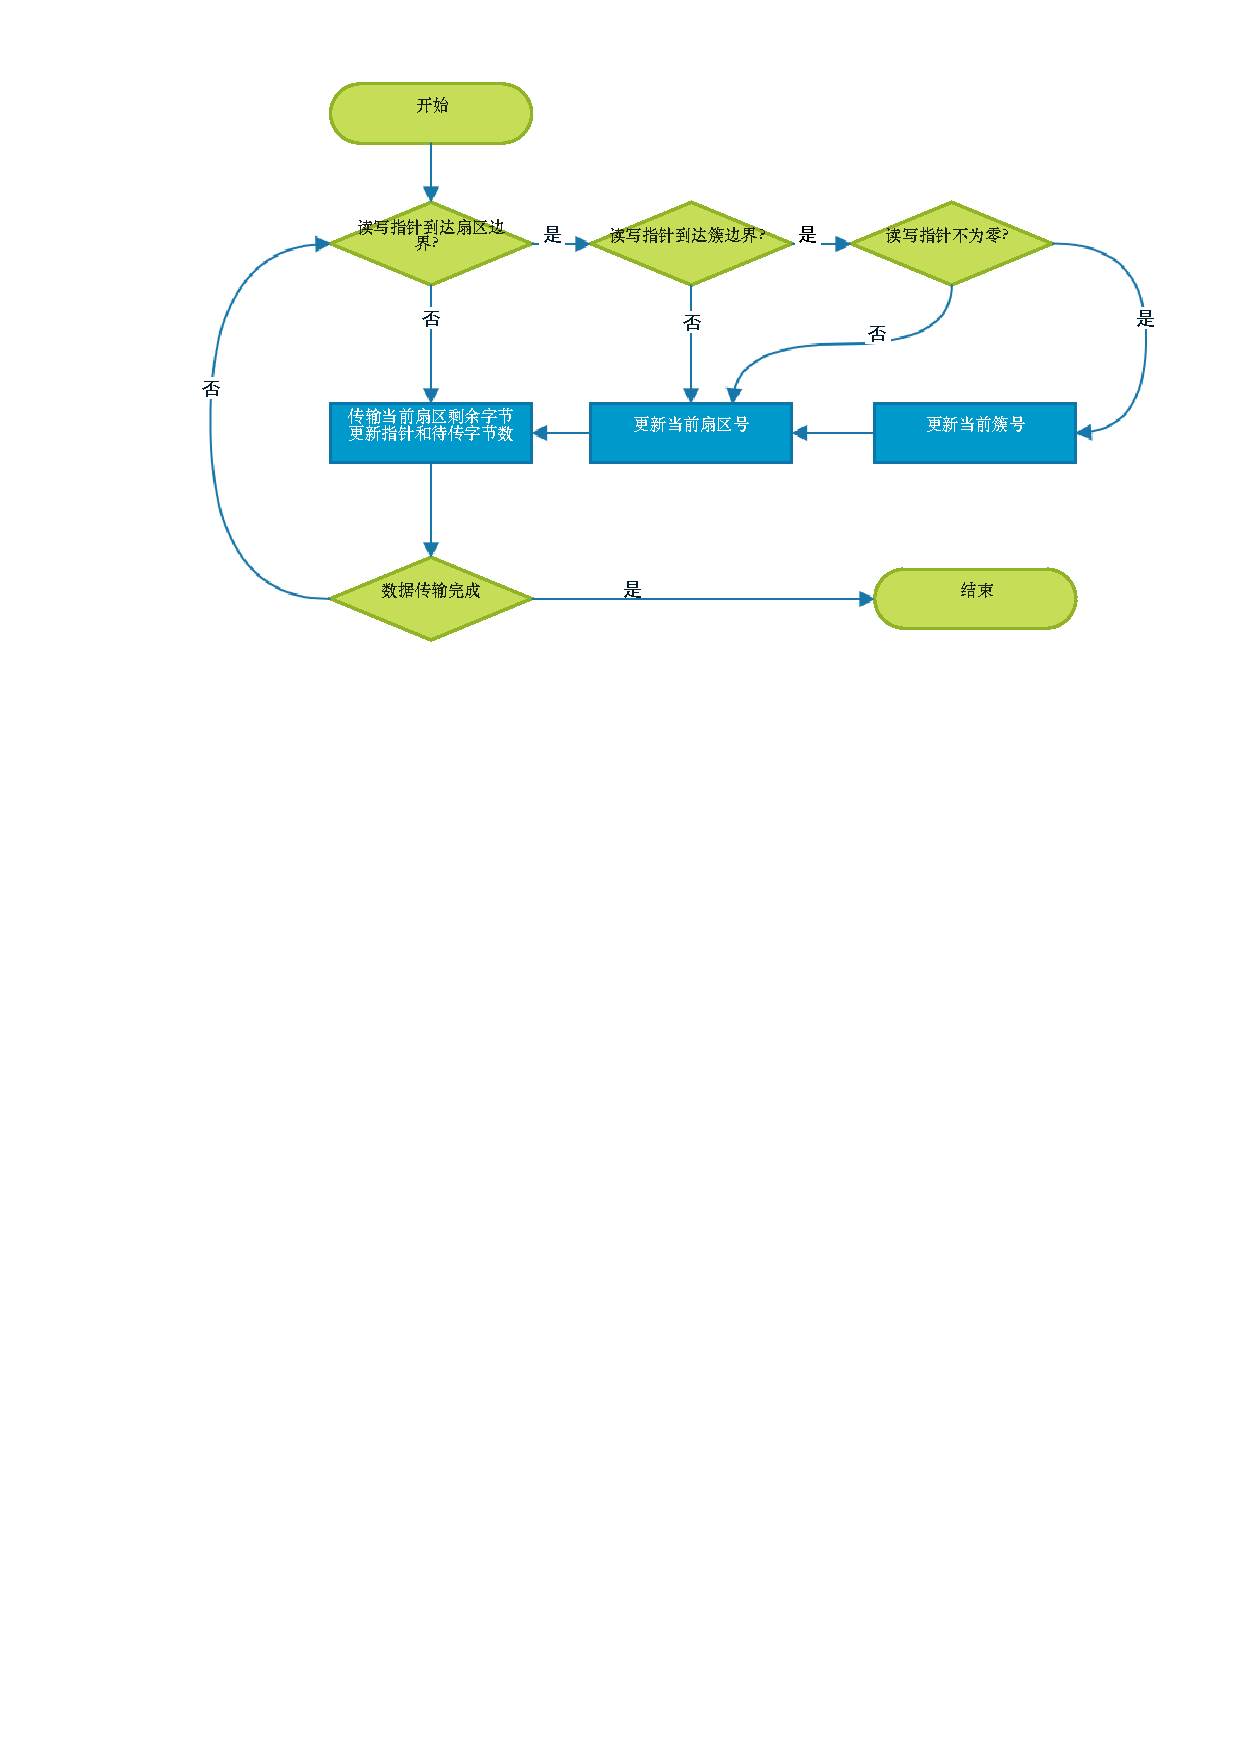
\includegraphics[width=1.0\textwidth]{chap3/freadh.pdf}
    \\
    \caption{读写文件}\label{fig:freadflow}
\end{figure}
读写文件整体上差不多,主体循环结构都如图\ref{fig:freadflow},主要差别在于其中的「更新当前簇号」操作。
在读文件操作中,更新簇号就是循着文件的簇链找到下一个簇号并使之成为当前簇号,赋值给「fs->curr\_clust」即可;
但在写文件操作中,更新簇号后还要求进一步判断:如果该簇号合法,则继续;如果该簇号为「EOC」标记,表明当前簇链已到末尾,
此时需要在该簇链的基础上创建簇链,即续接簇链,和之前的方法一样,找到一个空闲簇号,用其取代需要续接的簇链的最后一个簇号的值(「EOC」标记),
同时将该空闲簇号的值设为「EOC」标记即可,如此就完成了续链的操作。

\subsection{读写指针的重定位}
\label{sec:Ptr}
有时不想从文件的起始字节读写数据,而是想要向文件追加数据(从末尾写),或者修改文件中的某一部分数据(从文件中一个偏移值处写数据),此时,
就需要重定位文件的读写指针「fs->fptr」。
指针重定位函数不仅仅是重设了「fs->fptr」的数值,更重要的是,在重设指针的偏移字节后,要同时更新指针所在的扇区和簇号,以支持接下来的读写操作。

更新指针后,首先要通过「cnt $=$ (fs->fptr $\div$ fs->csize $\div$ 512)」求出在读写指针前有「cnt」个簇。
如果发现当前指针所在的簇为文件的第一个簇(cnt = $0$),
则将簇号回溯为文件的起始簇号即可。如果指针所在簇不是第一个簇(cnt $\neq 0$),那么需要通过起始簇号沿着簇链前进「cnt」次以取得相应簇号。

\section{底层函数的实现}
\label{sec:Diskread}
对于SD卡的驱动层模块,定义了一个32位长的全局变量$BASE$,用来记录逻辑扇区号与物理扇区号的差值。
当上层模块调用函数「disk\_offset()」时,将$BASE$的值设为「MBR」扇区「0x1C6」开始的32位数。
此后,对于上层的FAT模块,只需告诉底层模块逻辑扇区号即可,后者会在读写扇区前将之转化为物理扇区号。

\subsection{SD卡初始化并进入SPI模式}
\label{sec:Initial}
SD卡上电后处于SD模式,如果在接收复位命令(CMD0)期间片选信号(CS)保持低电平,那么将进入SPI模式。
如果卡检测到需求为SD模式则不会对复位命令做出响应,否则将切换至SPI模式同时回应SPI模式的R1。

返回SD模式的唯一方法是重新上电。在SPI模式中,所有SD卡协议的机器将不可见,而SD协议下的命令总是可用的。
图\ref{fig:specflow}显示了SPI模式的初始化序列。

初始化完成后需要通过CMD58的回应得到SD卡的CCS信息。当SD卡接受CMD8并且完成初始化后CCS有效。CCS=0表示其为标准容量卡,
CCS=1为大容量卡(SDHC或SDXC)。

\begin{figure}[!htbp]
    \centering
    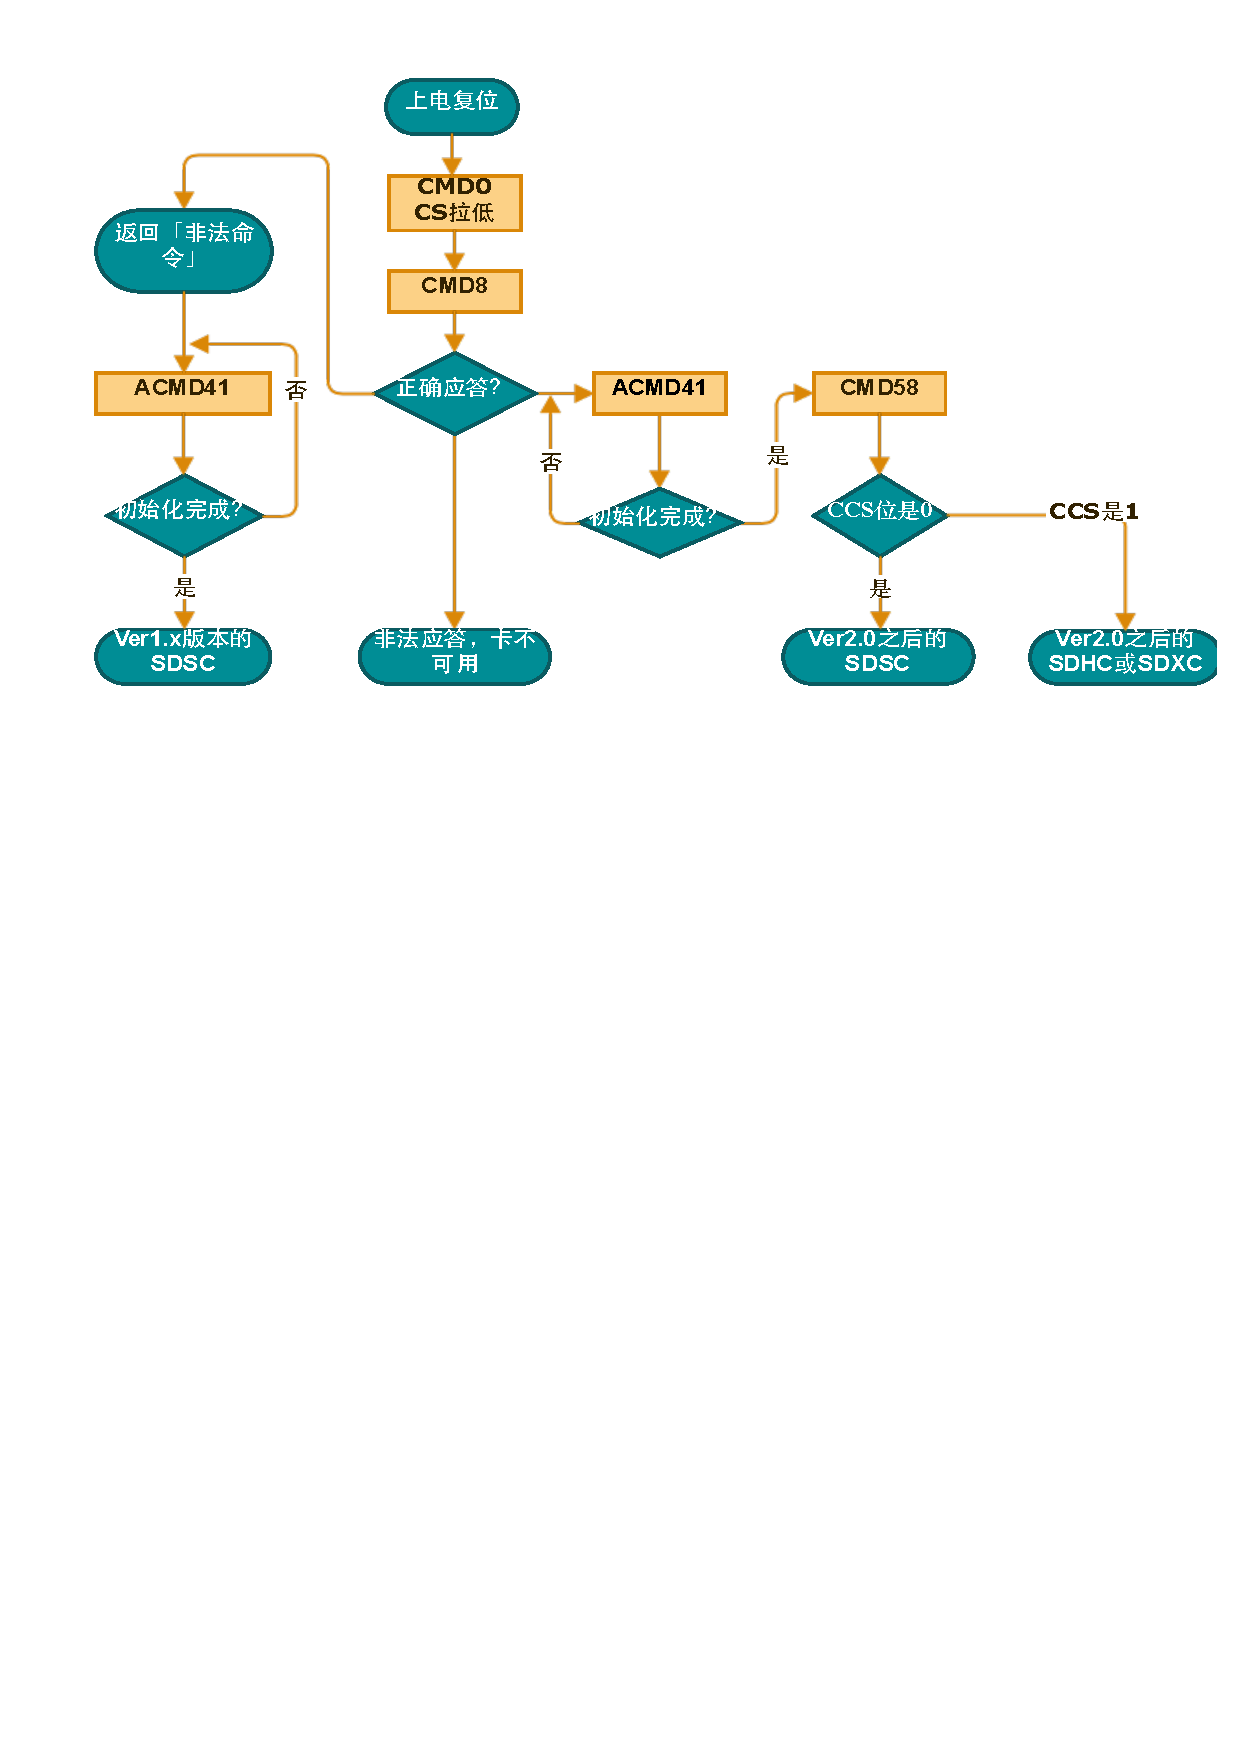
\includegraphics[width=1.0\linewidth]{chap3/specflowh.pdf}
    \\
    \caption{SPI模式初始化流程} \label{fig:specflow}
\end{figure}

初始化时需要采用低速初始化,此时SPI的时钟频率不能超过$400Khz$,本工程使用的是$200Khz$。
初始化结束后可以提升至高速。
发送命令后收到的响应如果不正确,可以循环发送命令直到收到正确应答。对于ACMD41而言,
由于其包含了两个命令(CMD55、ACMD41),故两个命令必需都收到正确应答才算响应正确,否则,两个命令都需要循环发送。

\subsection{SD卡读写扇区}
\label{sec:Sectorrw}
在SPI模式下读写扇区,首先要判断SD卡是SDSC还是SDHC/SDXC,对于前者,32位读写地址指的字节地址;对于后者,该地址指的是扇区地址。
为了同时兼容这两种卡,在该模块也定义了一个全局变量「SD\_Type」,在SD卡初始化函数中进行赋值,合法值为「SDSC」、「SDHC」和「SDXC」。
扇区读写函数通过下面方式选择字节地址或扇区地址。
\begin{lstlisting}[language={C}, caption={判断SD类型以选择合适的地址单位}]
if(*SD_Type != V2HC){
    sector = sector << 9;
}
\end{lstlisting}

由于不同文件系统的每簇扇区数各不相同,处于最大兼容性和效率性的考量,扇区读写函数都使用了单数据块传输的方式(512字节),因为一旦使用多数据块传输,
很可能出现跨簇的情况,这是非常危险的,因为本底层模块不具备跨簇的能力。
并且,本模块在写扇区之前,预先进行了擦除操作,这相比未擦除时的写入速度有了很大的提高。

\section{小结}
\label{sec:Sum3}
本章具体描述了整个文件接口各个模块的各功能函数的具体实现过程和方法,重点在与FAT文件系统模块的各个函数的实现过程,
为了增强可读性,极少使用伪代码描述,多数都采用自然语言的描述方式,与流程图相结合,具体阐述了功能的实现。


%==================================================
%% chapter03.tex for NWPU Bachelor Thesis
%% Encoding: UTF-8
%%==================================================

\chapter{实验与结果}
\label{chap:Results}
本FAT32文件系统接口的整体编译并导出HEX文件后,约占据16KB的代码空间,该模块运行时所需内存空间至少(512B + 100B),其中「512B」是缓冲池大小,
「100B」是各模块的全局变量总大小。然而在进行实验验证时,还需为需要读写文件操作另行开辟一块内存空间(512B),故实际所需内存空间至少为「1124B」。
同时为了实验的便利性,简化不必要的操作,使单片机与SD卡在SPI模式下通信,又为了尽可能提高读写速度,最好使用硬件SPI接口。
结合以上需求,本实验最终选择了C8051F020芯片,其有「4352B」的RAM,「64KB」的FLASH,并且带有一个硬件SPI接口,完全符合要求。

\section{工作区的文件组成}
\label{sec:Workspace}
考虑到本文件接口的模块化设计和实现,在实验验证过程也将分模块进行实验。
当对FAT文件系统模块进行实验时,底层的「disk.c」和「disk.h」将被测试用的测试文件「fattest.c」和「fattest.h」代替。
工作区文件构成如图\ref{fig:wsp1}。

\begin{figure}[!htbp]
    \centering
    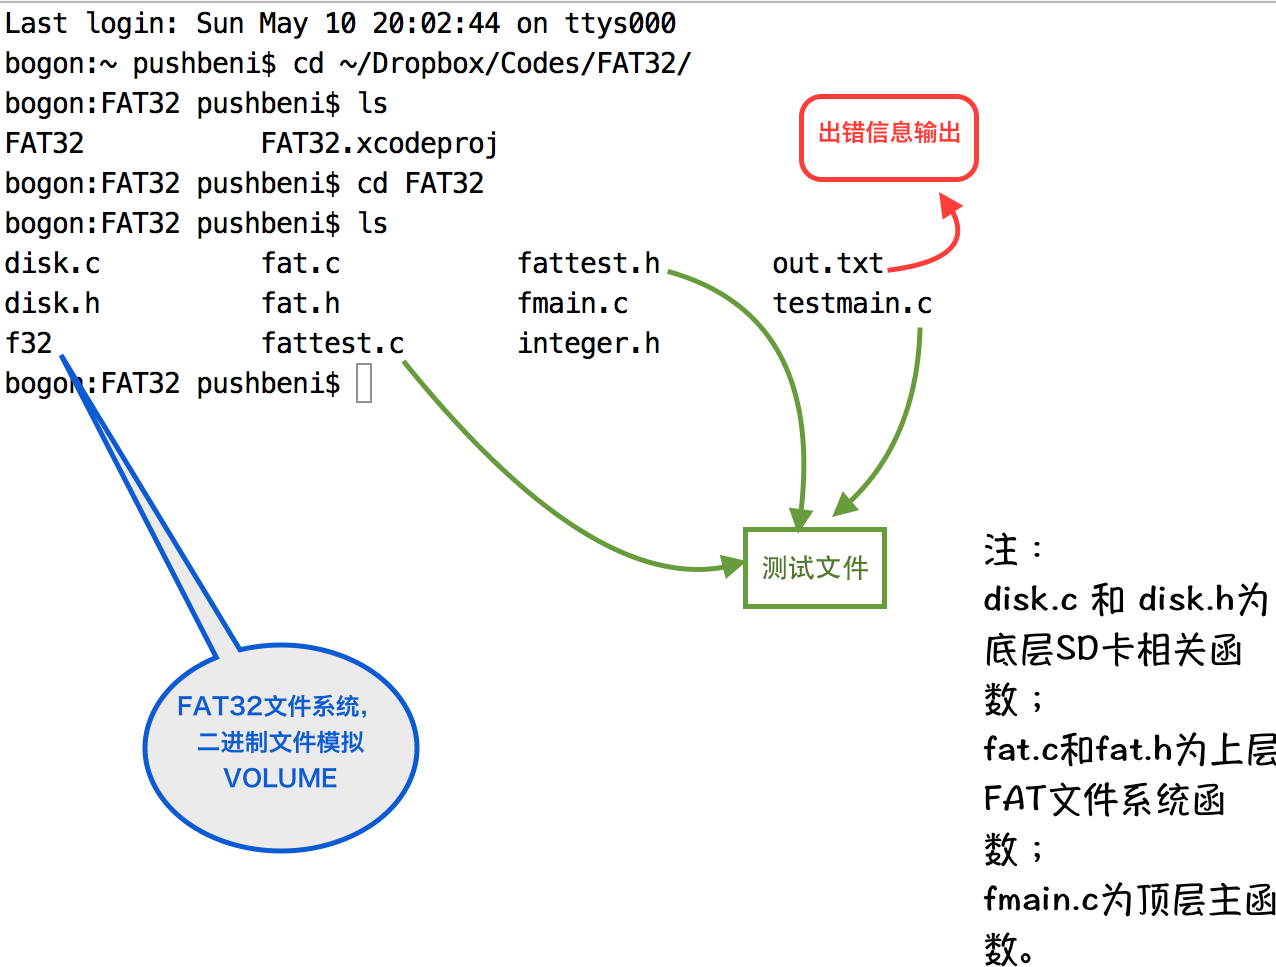
\includegraphics[width=1.0\linewidth]{chap4/workspace.png}
    \\
    \caption{工作空间} \label{fig:wsp1}
\end{figure}

其中的「f32」是一个二进制文件,用来模拟一个磁盘卷,以测试FAT模块的各项功能能否正确实现。「out.txt」是用来记录在FAT模块的各个函数换回值,
不仅用来记录出错信息,当FAT模块从“磁盘卷”(即「f32」文件)读出一个文件的数据后,测试程序会将读出的数据保存在这里供之后比对。
「testmain.c」就是在测试时的主程序,而「fmain.c」实际上就是「main.c」文件,是实际验证时的主程序文件。

当需要将两个模块组合在一起再次进行实际的实验时,
工作区的文件也要相应发送变化,之前的「fattest.c」和「fattest.h」将被真正的硬件层驱动函数「disk.c」所替换。
同时主文件也变成了「main.c」。
最终的工作区文件见图\ref{fig:wsp2}。
可以看到,本实验采用KEIL-C51进行源文件的编译并最终生成HEX文件烧如单片机,用C8051F的Debugger进行调试。

\begin{figure}[!htbp]
    \centering
    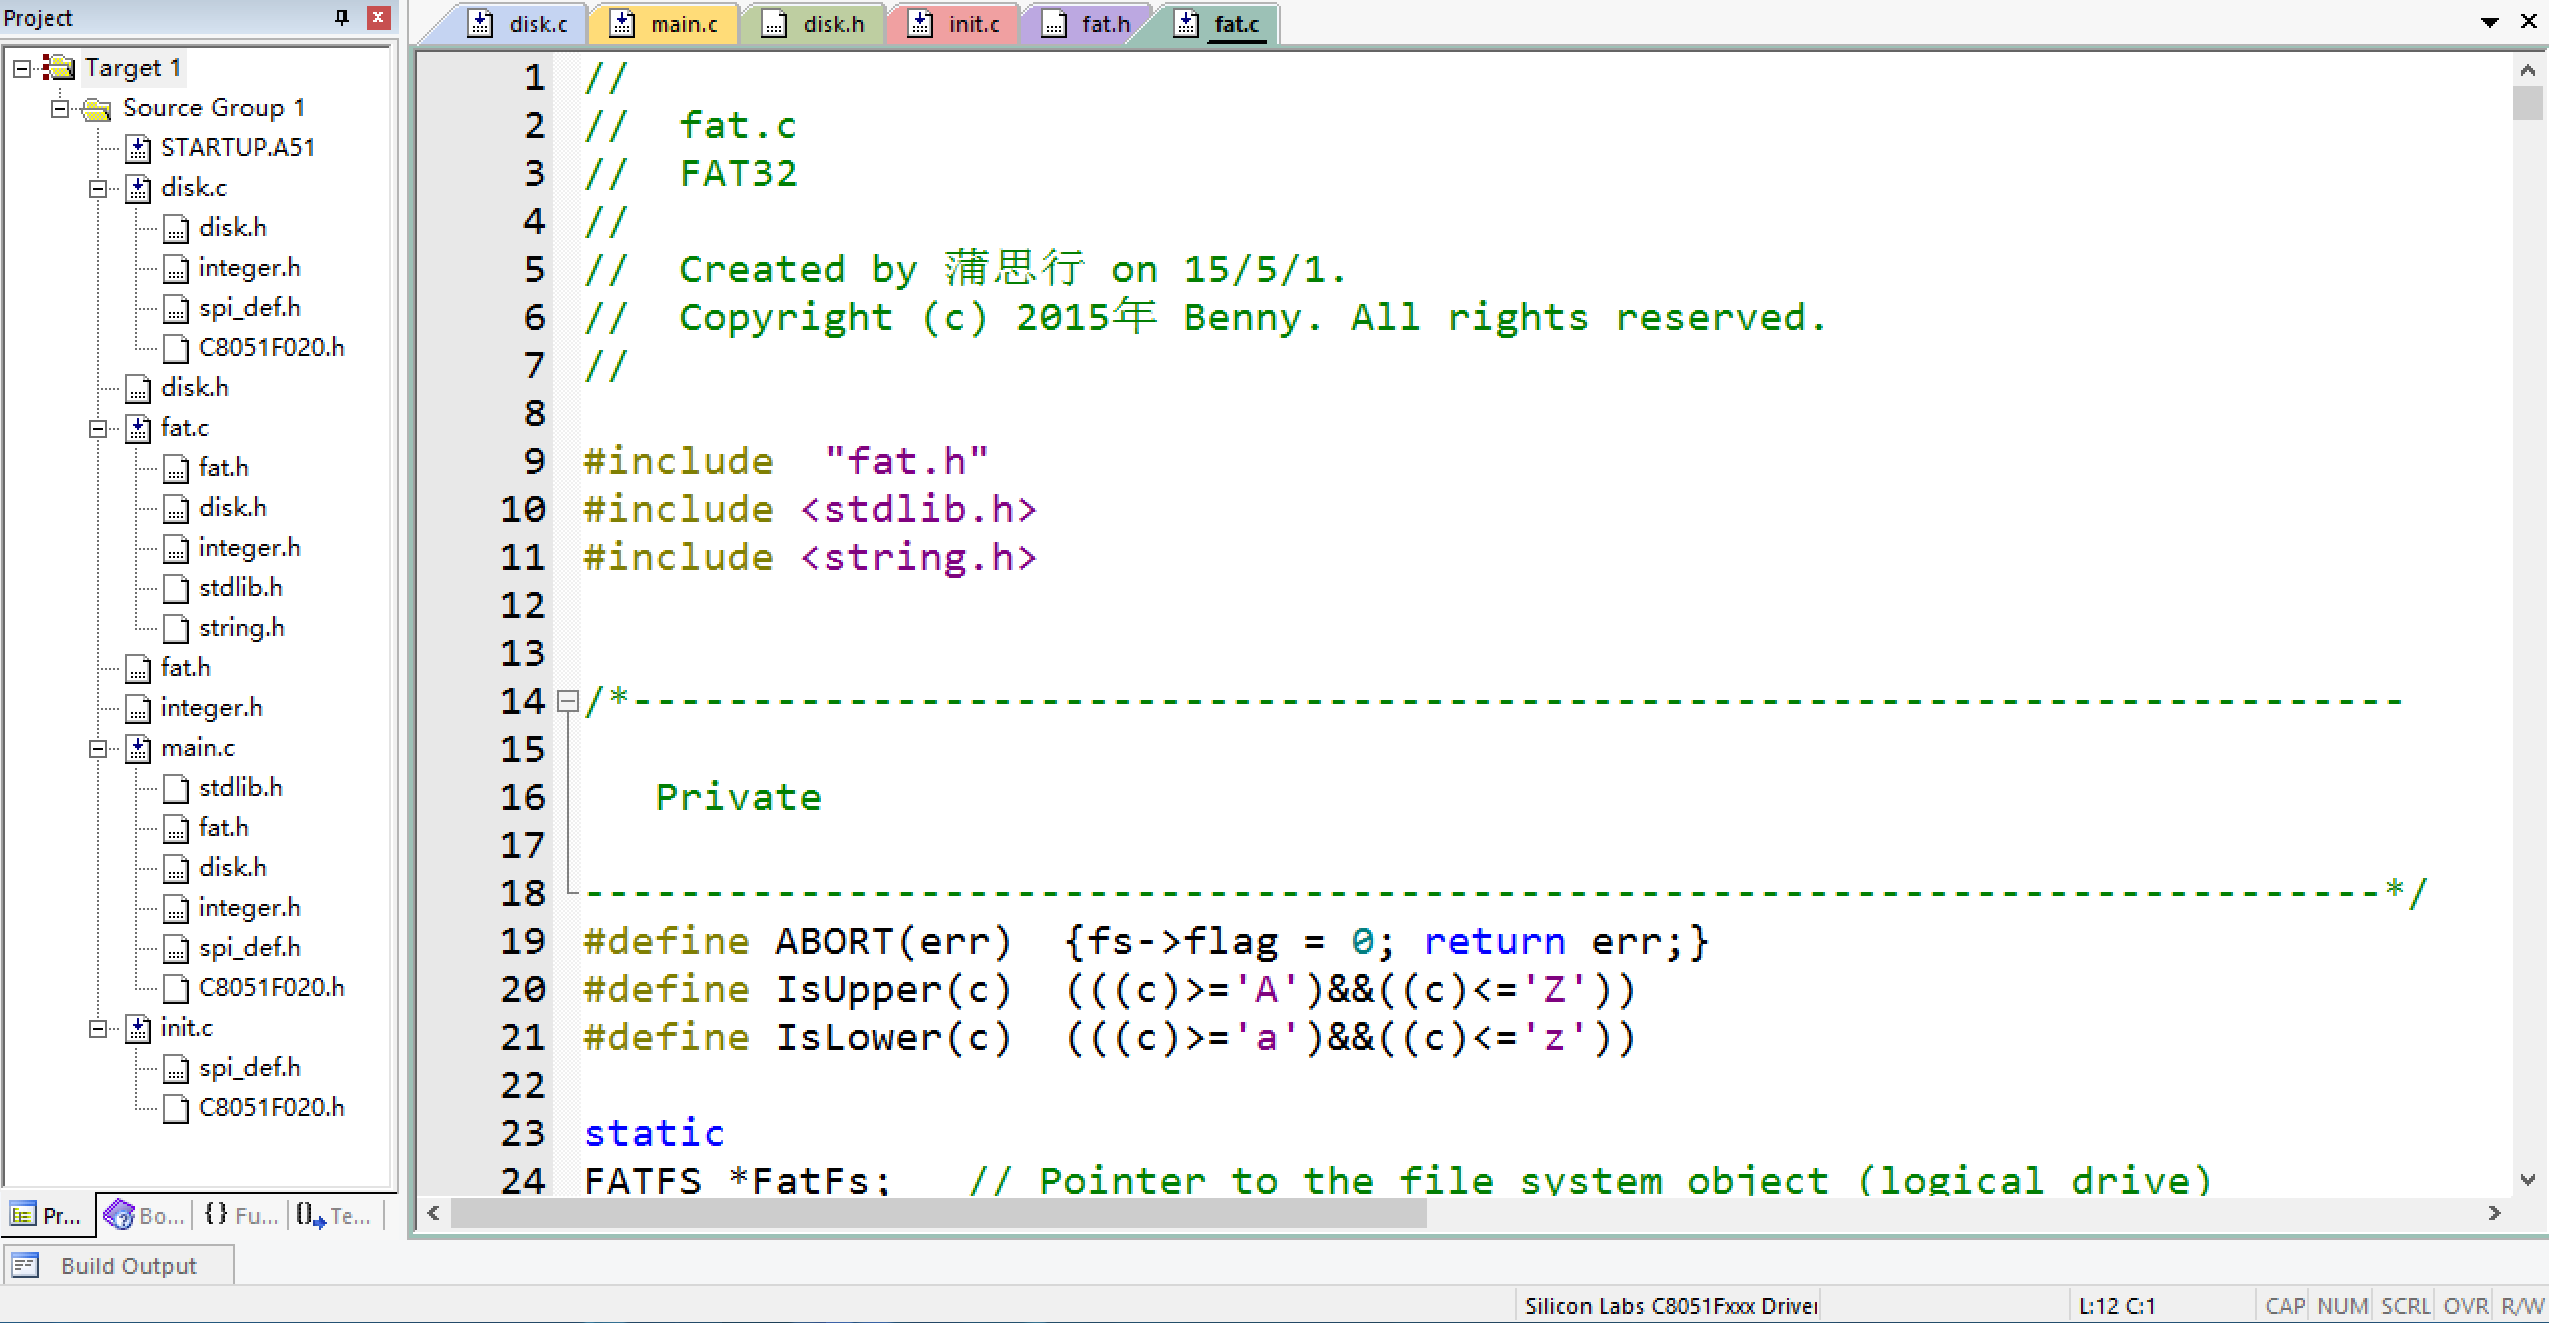
\includegraphics[width=1.0\linewidth]{chap4/workspace2.png}
    \\
    \caption{最终的工作空间} \label{fig:wsp2}
\end{figure}

\section{文件系统模块的逻辑验证}
\label{sec:ExpFAT}
文件系统模块的实验中,工作区如图\ref{fig:wsp1}。在这部分实验中,不需要考虑底层的情况,只需要相应函数功能在逻辑上能够正确无误的达成即可。
因此,为了模拟文件系统模块对物理磁盘的操作,实验时在磁盘上建立了一个无格式的二进制文件「f32」,用来模拟一个磁盘卷。当然,相应地,
测试文件「fattest.c」中的「disk\_\textit{xxx()}」之类的函数全部是通过「fopen()」、
「fread()」和「fwrite()」等函数\footnote{此处的「fopen()」等函数是在<stdio.h>中原生定义好的函数,用来实现对文件的操作,
不要与本文件接口定义的「f\_open()」等函数混淆}对文件进行操作。
但是在文件系统模块看来,好像是在对磁盘进行操作一样。

为了用「f32」二进制文件真正地模拟磁盘卷,首先要对它进行初始化配置,即将其“$0^{th}$”扇区(起始的512个字节)按照「DBR」启动扇区的格式填入正确的内容,
还要在“$1^{st}$”扇区按照正确的格式填入FSINFO扇区的内容。
配置好的「f32」文件如图\ref{fig:GUI}。

\begin{figure}[!htbp]
    \centering
    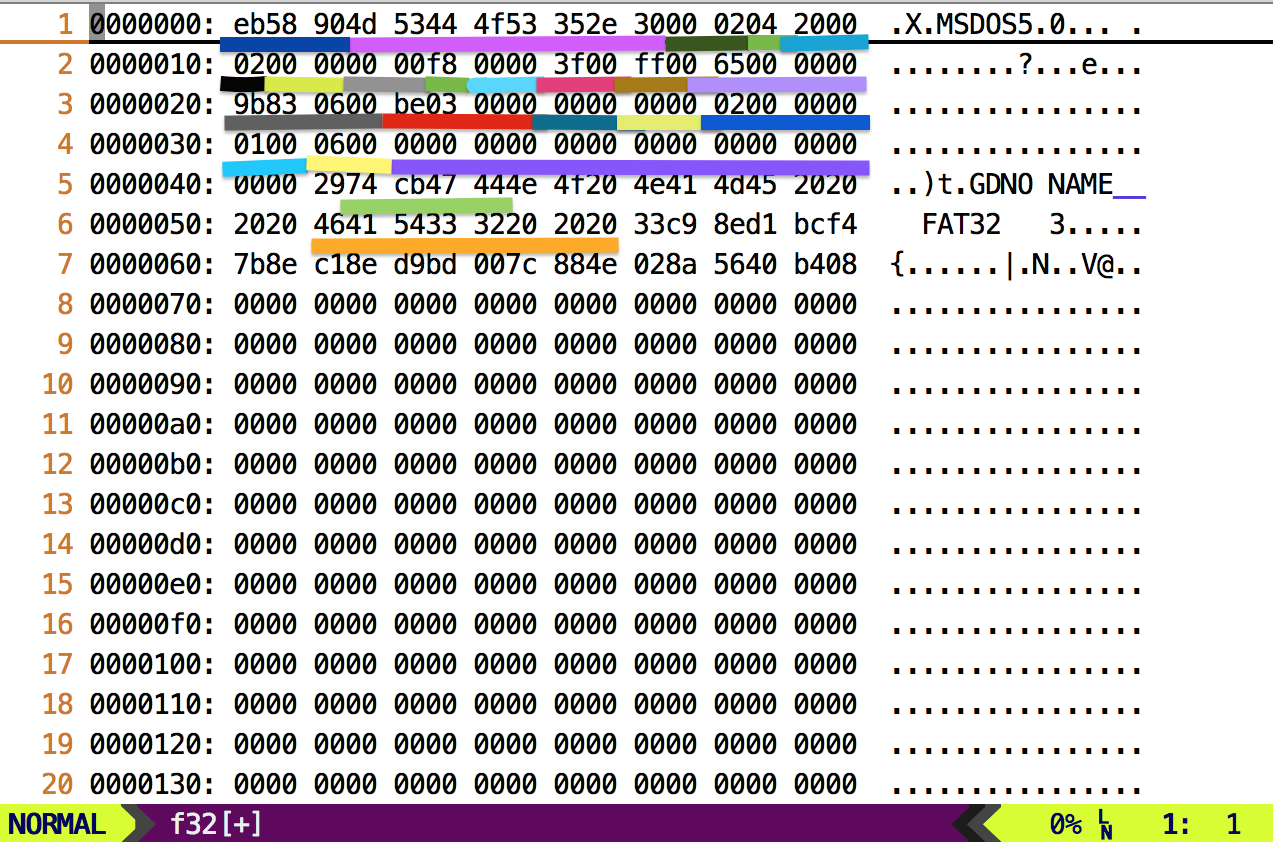
\includegraphics[width=1.0\linewidth]{chap4/GUI.png}
    \\
    \caption{模拟的启动扇区} \label{fig:GUI}
\end{figure}

文件系统挂载后,各项参数信息如图\ref{fig:mount}。
通过右下角的「lldb」调试信息可以看到,$*fs$的各项信息已经有了正确的值,并且从「res=FR\_OK」也知道了磁盘卷已经正确挂载。
可以看到,测试用的模拟的磁盘卷的簇大小为4个扇区,即2KB,「fs\_type」为「0x33」表是该文件系统是FAT32,
「fatbase」为「32」表示FAT表的起始扇区是32号扇区,即第「0x4000」字节处。「dirbase」为「2」表示根目录起始簇为2号簇,即第「0xF3800」字节处。

\begin{figure}[!htbp]
    \centering
    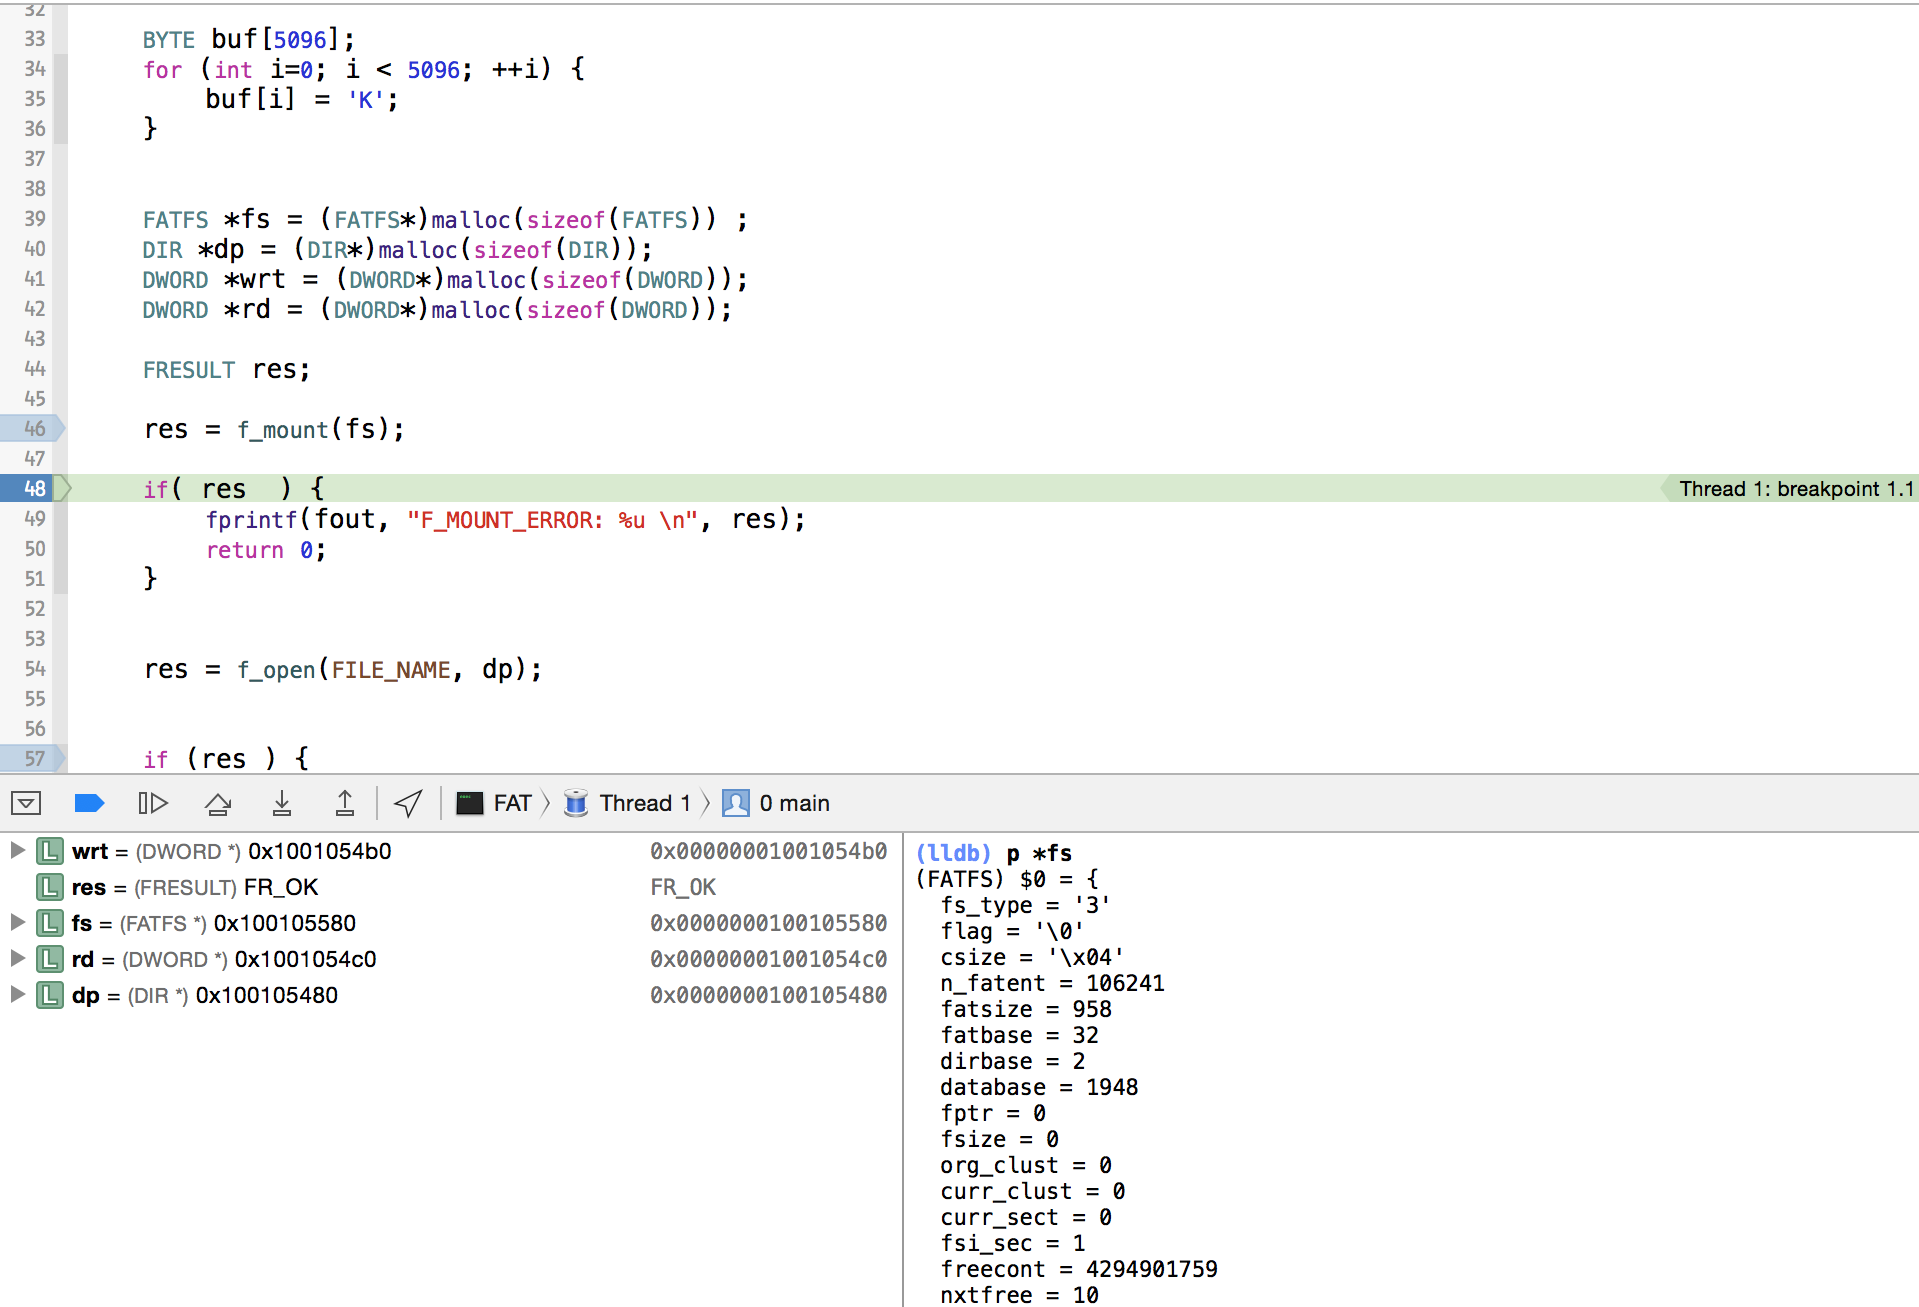
\includegraphics[width=1.0\linewidth]{chap4/mount.png}
    \\
    \caption{挂载文件系统} \label{fig:mount}
\end{figure}

接下来可以在根目录新建一些文件「TEXT1.TXT」、「TEXT2.TXT」和「TEXT3.TXT」,
新建文件操作后结果如图\ref{fig:dircrt}。

\begin{figure}[!htbp]
    \centering
    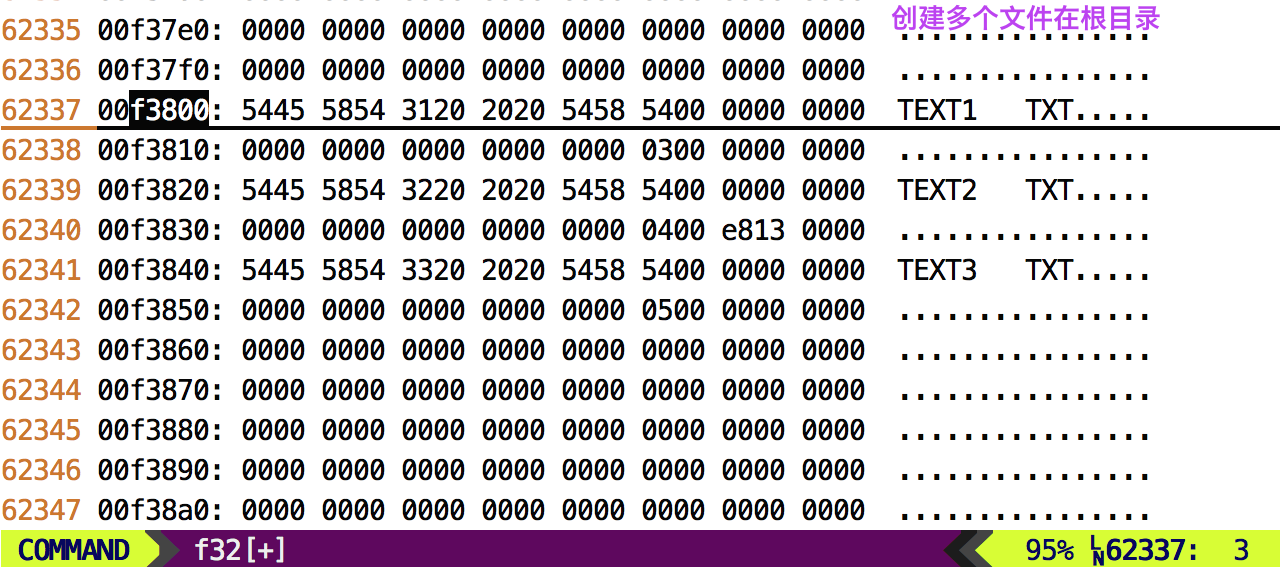
\includegraphics[width=1.0\linewidth]{chap4/dircrt.png}
    \\
    \caption{目录表中新建目录项} \label{fig:dircrt}
\end{figure}

之后进行写操作,写入超过一簇(如5096个字节)的数据后,FAT表会更新并续接簇链,写入后更新的FAT表如图\ref{fig:fatcrt}。

\begin{figure}[!htbp]
    \centering
    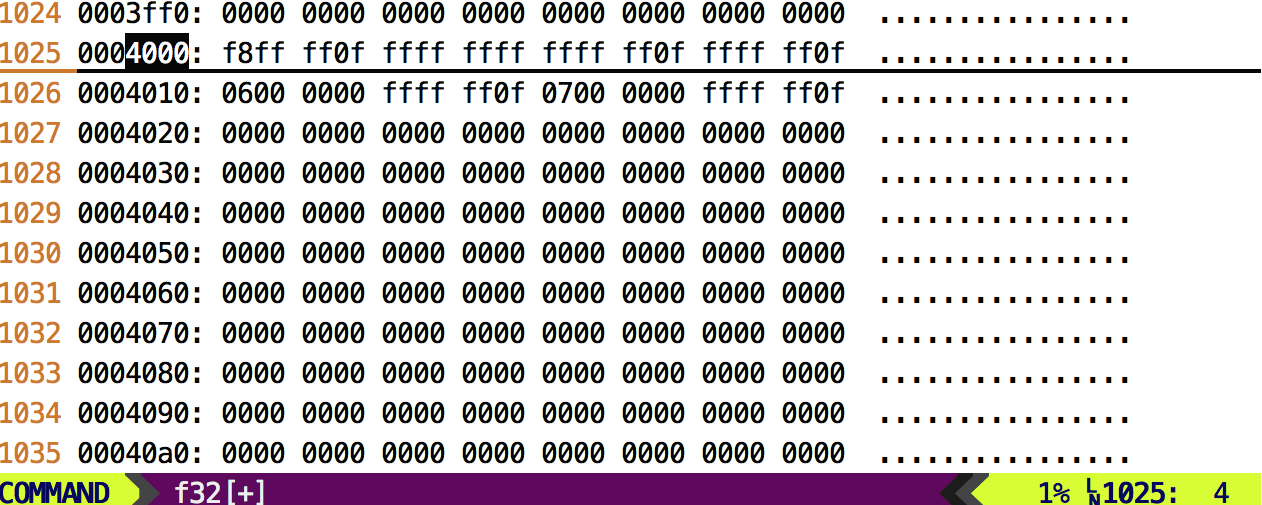
\includegraphics[width=1.0\linewidth]{chap4/fatcrt.png}
    \\
    \caption{FAT表分配新的簇号} \label{fig:fatcrt}
\end{figure}

写入数据后,磁盘卷的数据区如图\ref{fig:datawrt}

\begin{figure}[!htbp]
    \centering
    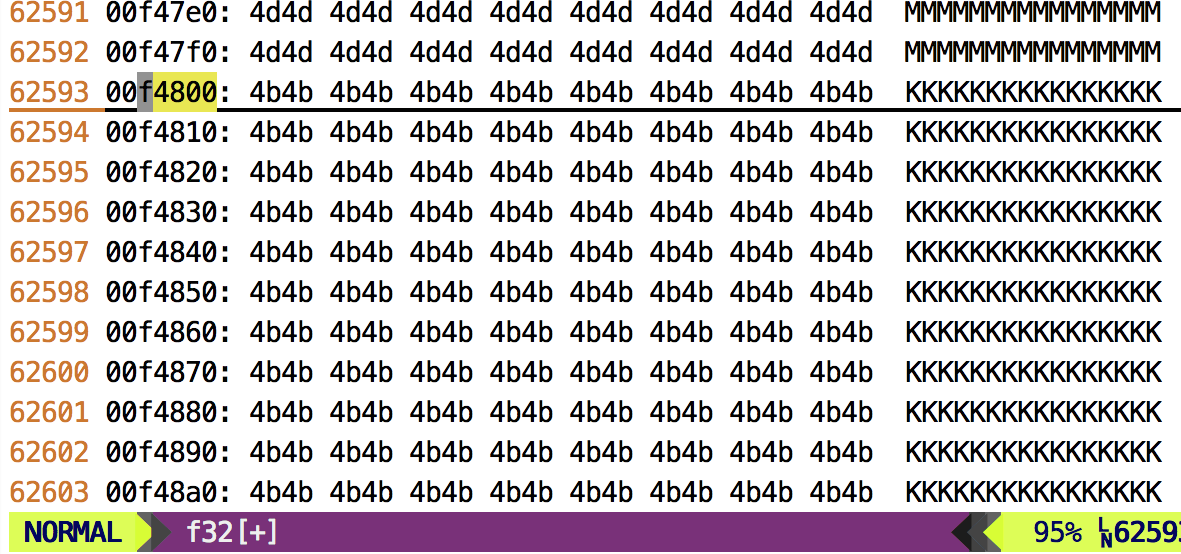
\includegraphics[width=1.0\linewidth]{chap4/datawrt.png}
    \\
    \caption{写入后的磁盘卷数据区} \label{fig:datawrt}
\end{figure}

当成功写入文件后,还要再测试从文件读取数据的过程,正确读取后返回值应为「FR\_OK」,同时缓冲池「buf」中应该有正确的数据,结果如图\ref{fig:datard}。

\begin{figure}[!htbp]
    \centering
    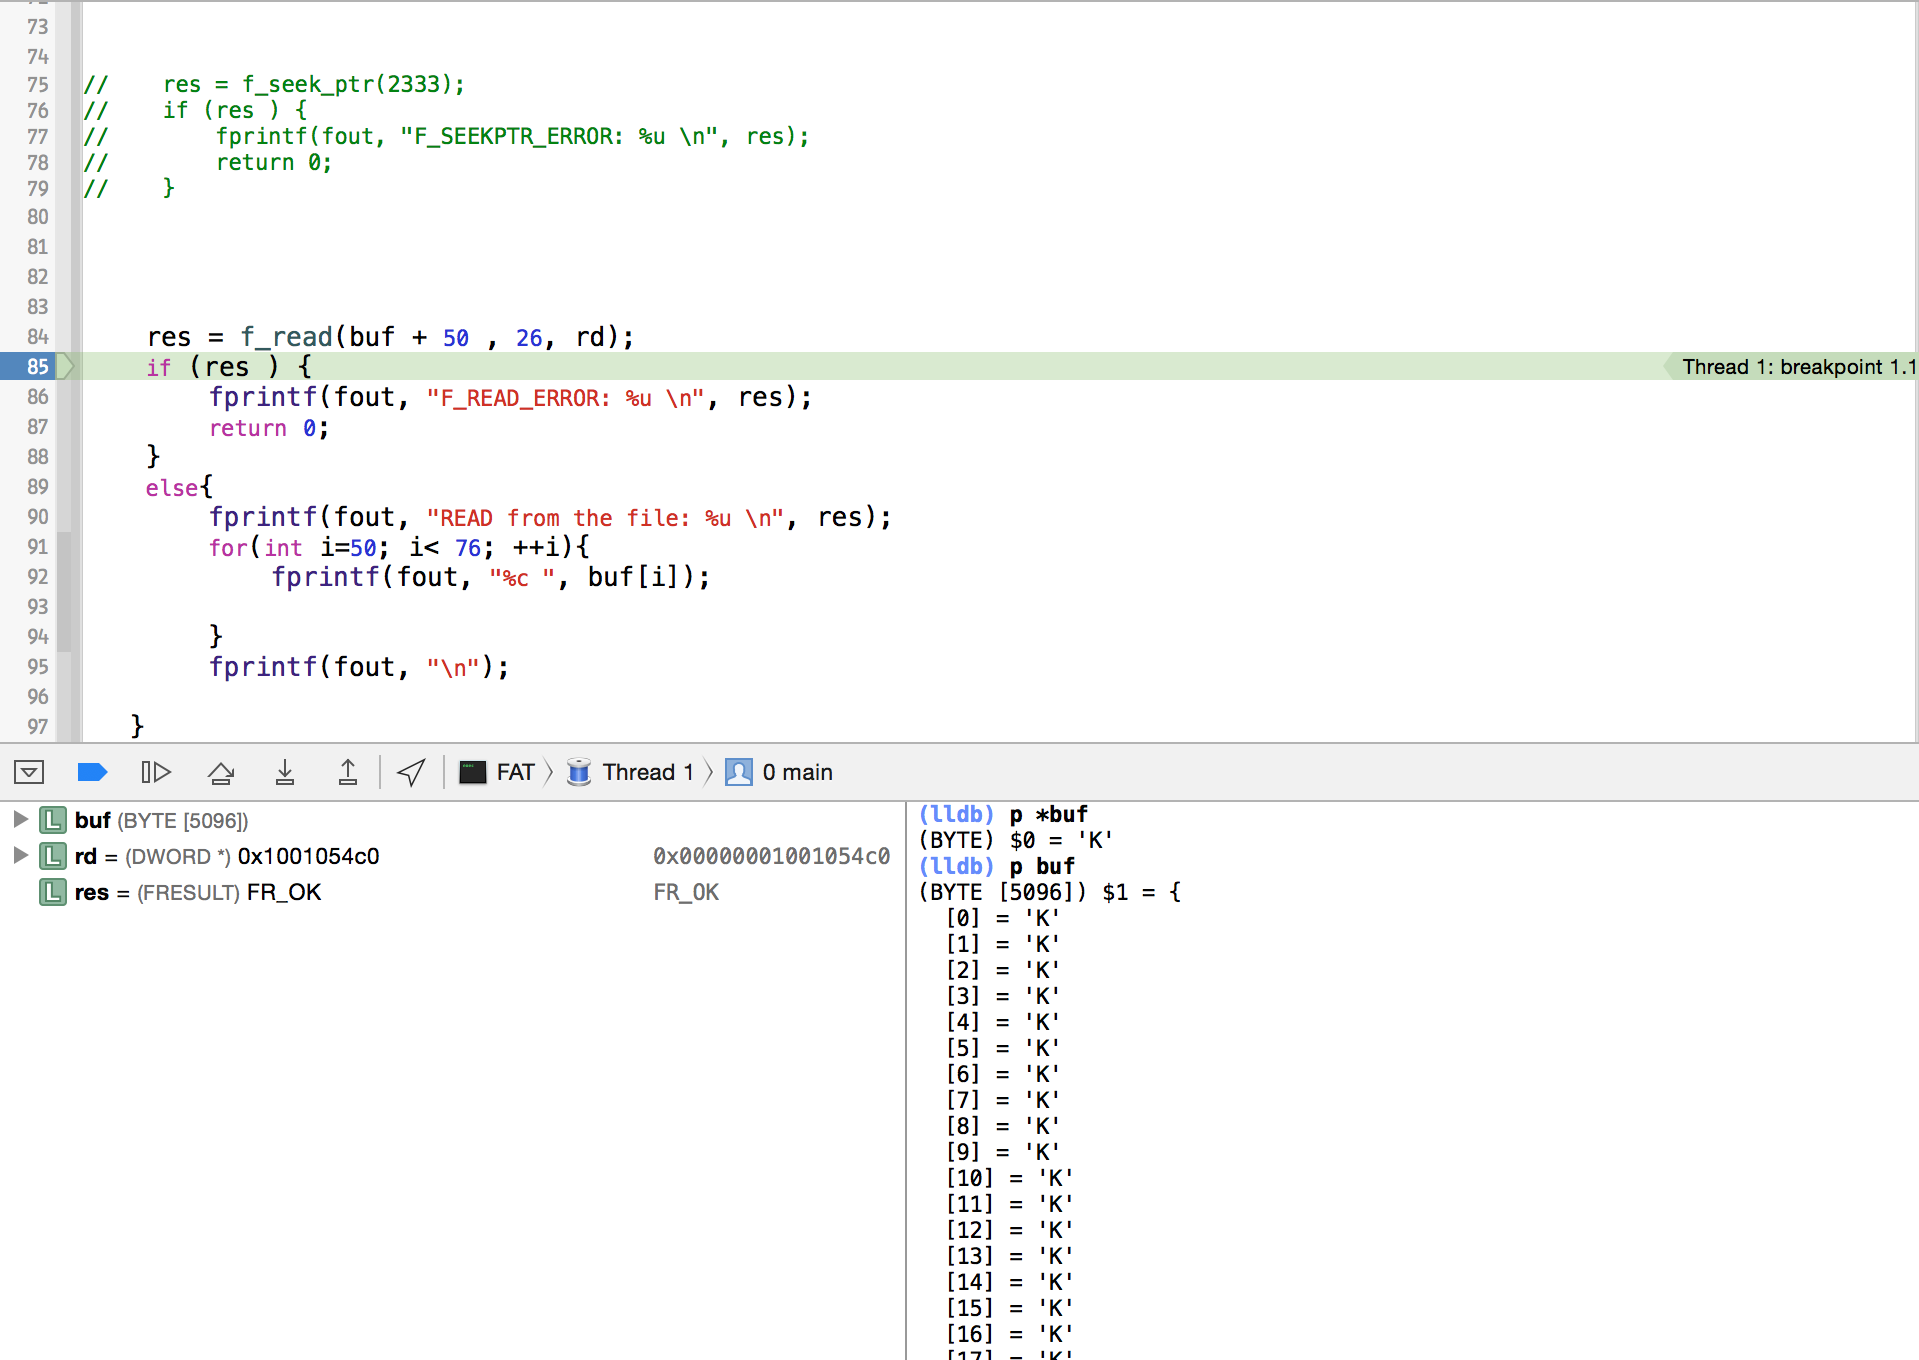
\includegraphics[width=1.0\linewidth]{chap4/datard.png}
    \\
    \caption{读文件的结果} \label{fig:datard}
\end{figure}

最后的实验项目是删除文件,删除文件不仅要删除目录表的记录,还要清除FAT表的相应簇链。
删除后结果如图\ref{fig:dirrm}和\ref{fig:fatrm}。

\begin{figure}[!htbp]
    \centering
    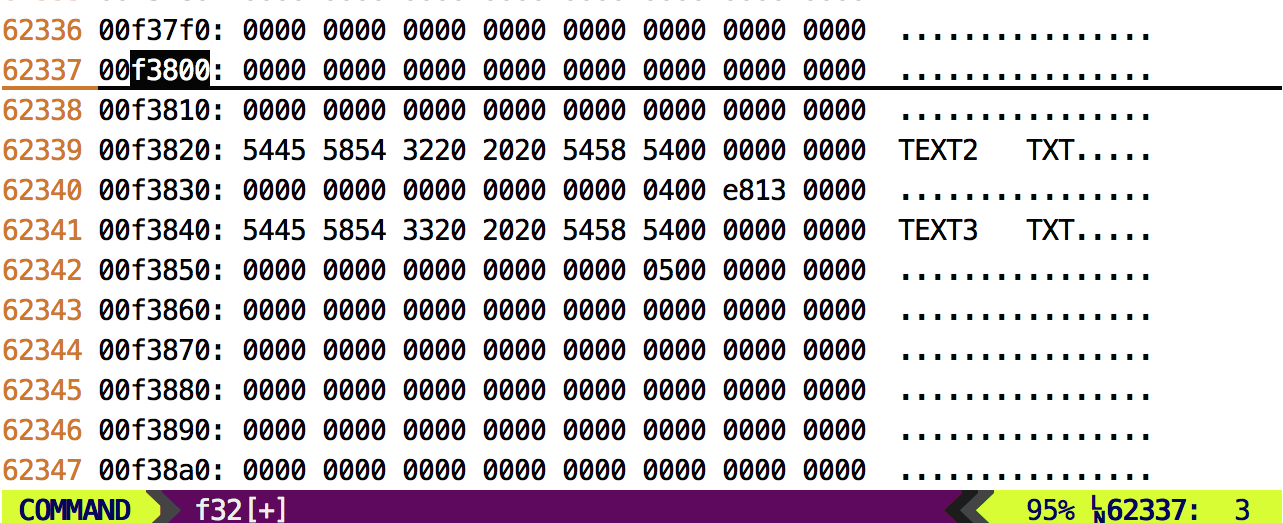
\includegraphics[width=1.0\linewidth]{chap4/dirrm.png}
    \\
    \caption{删除后的目录表} \label{fig:dirrm}
\end{figure}

\begin{figure}[!htbp]
    \centering
    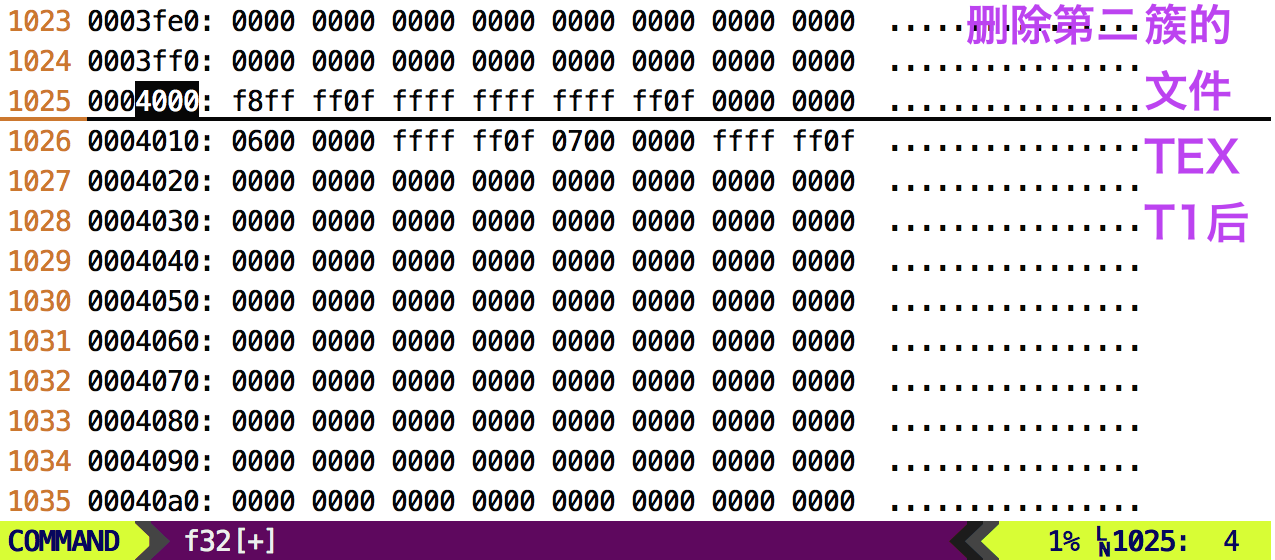
\includegraphics[width=1.0\linewidth]{chap4/fatrm.png}
    \\
    \caption{删除后的FAT表} \label{fig:fatrm}
\end{figure}

\section{实际的实验验证}
\label{sec:ExpDriver}
整个文件接口的实现过程必须和底层的硬件相契合,对于不同的硬件或者不同的环境,都要求做出相应的调整。
本工程实现过程中用到了以C8051F020为MCU的单片机,同时用到了一个SD卡槽,该卡槽是11脚卡槽。

实验测试的SD卡是一张4GB的SDHC卡,实际上本接口能够支持几乎所有类型的SD卡,即使是老版本(Version 1.x)的老式卡也没有问题。
实验用到的板子如图\ref{fig:mcu}和\ref{fig:11sd}所示。鉴于本实验只需使用C8051F020的「P0.0」-「P0.3」引脚,再加一根片选线「CS」,本实验将其分配给了「P3.1」。
硬件SPI的「P0.3」是「NSS」位,是输入信号,只做从机片选,不能用做CS输出片选,因此要将它始终拉高(不使能)。

由于微处理器所在的板子没有SD卡槽,故另外引了4根数据线到图\ref{fig:11sd}中的SD卡槽。
该11脚的SD卡槽,
比正常的9脚SD卡多了两个保护引脚,其中一个保护引脚是卡插入检测位「CD」,
然而该引脚并没有接在SD卡的「CD/DAT3」引脚上。对于11脚的卡槽,「DAT3」脚与SD卡的「CD/DAT3」相连接。
在程序运行中,本接口通过判断「CD」引脚的电平高低来进行SD卡的插入拔出检测,当SD卡正确插入后,「CD」被拉低,否则其始终为高电平。

\begin{figure}[!htbp]
    \centering
    \includegraphics[width=1.0\linewidth]{chap4/mcu.png}
    \\
    \caption{C8051F020} \label{fig:mcu}
\end{figure}

\begin{figure}[!htbp]
    \centering
    \includegraphics[width=1.0\linewidth]{chap4/11sd.png}
    \\
    \caption{SD卡槽} \label{fig:11sd}
\end{figure}

整体的实验环境如图\ref{fig:vol}

\begin{figure}[!htbp]
    \centering
    \includegraphics[width=1.0\linewidth]{chap4/vol.png}
    \\
    \caption{硬件环境} \label{fig:vol}
\end{figure}

在SD卡中新建「TEXT6.TXT」等文件后,将SD插入PC机,可以识别。
并且「TEXT6.TXT」文件被写入了37KB的数据用来测试跨簇大文件的支持程度,而「TEXT1.TXT」仅写入了4KB数据,
「TEXT10.TXT」是新创建的文件,还没有写入数据。

\begin{figure}[!htbp]
    \centering
    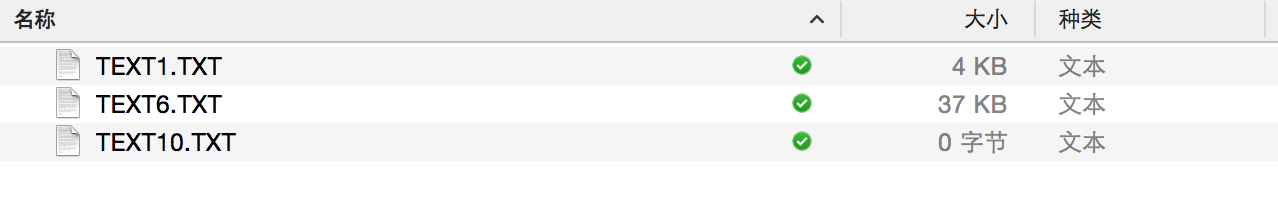
\includegraphics[width=1.0\linewidth]{chap4/sdwrt.png}
    \\
    \caption{SD卡插入PC后} \label{fig:sdwrt}
\end{figure}

为了测试大文件写入过程是否顺利,但是单片机有没有足够大的内存空间,故选择了使用同一个缓冲池循环写入。同时为了快速更换缓冲池的内容,
直接通过「memset()」函数对其赋值。

\begin{figure}[!htbp]
    \centering
    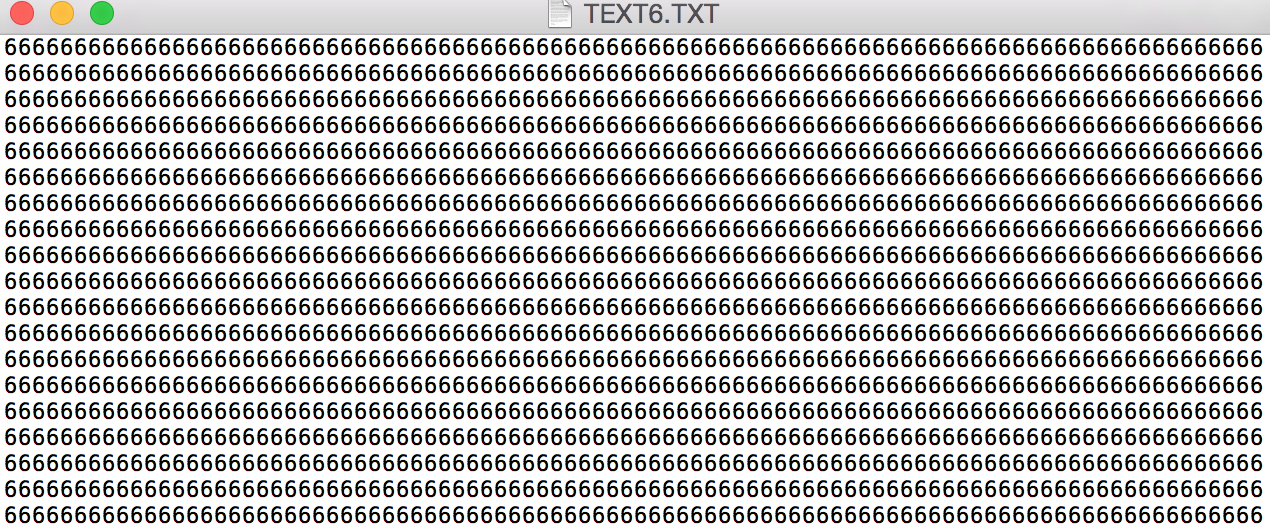
\includegraphics[width=1.0\linewidth]{chap4/sddata.png}
    \\
    \caption{写入长数据后文件的内容} \label{fig:sddata}
\end{figure}

可以看到,计算机是能该正确读取单片机向SD卡的文件中写入的数据的。

\section{结果}
\label{sec:Conclusion}
通过本次的实验和验证,成功完成了本FAT32文件接口对以SD卡为介质的文件系统的操作。
单片机通过本文件接口,实现了对FAT文件系统的挂载,能够在根目录新建文件和删除文件,
并且能够打开文件进行读写操作,跨簇的大文件长文件也完全没有问题。

预期的要实现的目标包括文件系统挂载、SD卡插拔检测、文件的新建与删除、打开关闭文件及读写文件等功能均能够顺利实现,
并且本接口还能够在文件的特定位置读写文件。

上述的各项操作都是以FAT32文件系统的规范为标准,完全契合并兼容FAT32文件系统,使得计算机在插入SD卡后,能够浏览根目录下的单片机所创建的各项文件,
并且也能够正确识别并打开这些文件进行读取和修改,这使得单片机与计算机的协同工作能力得到极大的提升,二者的联系更为密切,
它们之间进行数据共享可以通过SD卡方便的完成。

\section{小结}
\label{sec:Sum4}
本章详细描述了具体的实验过程及实验验证结果,首先进行上层FAT模块的逻辑实验验证,仅验证测试其逻辑功能。然后,当模块化测试通过后,
在使之与底层的SD卡驱动模块结合起来进行联合调试,在具体的实际操作中进行实验验证。
最终结果显示整个文件接口符合要求,各预期功能顺利达成。

%%==================================================
%% conclusion.tex for SJTUThesis
%% Encoding: UTF-8
%%==================================================

\chapter{全文总结}
\label{chap:Summary}

本文详细描述了基于微处理器的FAT32文件接口的设计与实现过程,
而该文件接口解决了单片机难以通过SD卡与计算机通信的问题,

通过对FAT文件系统和SD卡的SPI模式的学习和理解,阅读大量资料后,完成了文件接口的设计,
并最终在单片机上实现了该设计。
本文件接口在底层实现了单片机通过SPI总线协议与SD卡的数据传输,借助11脚SD卡槽,
能够对SD卡进行插拔检测,同时,能够识别并支持不同版本和容量的SD卡,无论是Version 2.0以后的卡还是Version 1.x的老式SD卡,无论是SDSC、SDHC还是SDXC均能正确识别并读写数据。
在SPI模式下,SPI总线时钟决定了数据的传输速率。本实验采用了C8051F020芯片,
其内置晶振最高$16Mhz$,而SPI的总线时钟最高为$8Mhz$,故在理想情况下\footnote{
    所有比特位都正确的传递,所有命令都能够无误收发},通过SPI协议与SD卡通信能够达到
的最大速率是$1MB/sec$\footnote{同前,此处的「MB」指1000 $\times$ 1000 Bytes}。

本文件接口最重要最核心的部分在于上层FAT模块的设计,该模块具有良好的可移植性,
通过隐藏不必要的程序接口实现了良好的稳定性。
该模块能够正确识别磁盘的「MBR」和「DBR」扇区,对于SD卡而言,通常只存在一个卷,且该卷
的起始扇区号被记录在整个磁盘的物理$0^{th}$扇区中,该FAT模块能够准确判断并迅速找到
SD卡的文件卷的真正起始扇区,不必一个扇区一个扇区地逐个判断,这加快了文件系统的挂载速度。
该模块实现了在根目录下对文件的创建、打开、写入、读取等一系列操作,同时支持「FSINFO」
数据结构,并且,通过「直写」(Write Through)的方式操作磁盘与内存的数据交换,
简化了结构的复杂度,实现了更好的兼容性,无需考虑同步问题。

当然,本工程仍然存在着待改进的地方,比如尚未实现对长文件名(LFN)的支持,
目前只能在根目录区操作等。

总之,本文件接口解决了单片机通过SD卡与计算机的数据共享问题,通过该接口可以
方便地向SD中存储数据或者读出数据,实现了兼容性,扩大了单片机的适用范围和用途。



\appendix   % 使用英文字母对附录编号,重新定义附录中的公式、图图表编号样式
\renewcommand\theequation{\Alph{chapter}--\arabic{equation}}	
\renewcommand\thefigure{\Alph{chapter}--\arabic{figure}}
\renewcommand\thetable{\Alph{chapter}--\arabic{table}}
\renewcommand\thealgorithm{\Alph{chapter}--\arabic{algorithm}}


\backmatter	% 文后无编号部分 

%% 参考资料
\printbibliography[heading=bibintoc]
%\bibliography{bib/fat.bib}

%% 致谢、发表论文、申请专利、参与项目、简历
%% 用于盲审的论文需隐去致谢、发表论文、申请专利、参与的项目
\makeatletter
\ifsjtu@review\relax\else
    %%==================================================
%% thanks.tex for SJTU Master Thesis
%% based on CASthesis
%% modified by wei.jianwen@gmail.com
%% version: 0.3a
%% Encoding: UTF-8
%% last update: Dec 5th, 2010
%%==================================================

\begin{thanks}

  感谢指导教师陶林伟老师的指导与点拨!在本工程的调试与测试中给予很多帮助!

  感谢@ChaN的FatFs文件系统的启发!

  感谢StackOverFlow上的热情帮助的友人!在这里帮助我解决了很多问题!

  感谢诸位同学的热情帮助!
  

\end{thanks}
           %% 致谢
    \begin{grasum}
    历时半年的本科毕业设计终于告一段落。

    在仔细地学习研究并理解FAT官方文档后,我终于能够亲手做出FAT32的文件接口了,尽管有些地方还不够完善,
    但毕竟实现了预期的功能,我还是比较满意的。在这半年中,我通过网路查阅了大量资料,
    当然,主要的、根本的参考资料是官方文档(分别来自Microsoft Coporation 和 SD Group),
    上百页的资料都需要仔细阅读、理解。
    同时我还参考了@ChaN的FatFs开源项目,学习到了文件系统的整体设计思路,获益匪浅。

    通过毕业设计的锻炼,在具体实践的过程中,我对FAT文件系统和SD卡都有了深刻的了解,
    尤其是对文件系统有了更本质、更底层、更具体的理解。并且,通过完成实际项目,我也认识到了理论与实践的距离,
    完美的理论也需要可操作的实验验证,上层设计终究要与底层硬件模块相结合才能实现所需要的功能。
    
\end{grasum}
        %% 毕业小结(Bachelor)
%   %%==================================================
%% pub.tex for SJTUThesis
%% Encoding: UTF-8
%%==================================================

\begin{publications}{99}
    \item\textsc{Chen H, Chan C~T}. {Acoustic cloaking in three dimensions using acoustic metamaterials}[J]. Applied Physics Letters, 2007, 91:183518.
    \item\textsc{Chen H, Wu B~I, Zhang B}, et al. {Electromagnetic Wave Interactions with a Metamaterial Cloak}[J]. Physical Review Letters, 2007, 99(6):63903.
\end{publications}
           %% 发表论文
%   \begin{patents}{99}
    \item 第一发明人,“永动机”,专利申请号202510149890.0
\end{patents}
       %% 申请专利
%   %%==================================================
%% projects.tex for SJTUThesis
%% Encoding: UTF-8
%%==================================================

\begin{projects}{99}
    \item 973项目“XXX”
    \item 自然基金项目“XXX”
    \item 国防项目“XXX”
\end{projects}
      %% 参与的项目
%   \include{tex/resume}        %% 各人简历
\fi
\makeatother

%% 附录内容,本科学位论文可以用翻译的文献替代。
%%==================================================
%% Encoding: UTF-8
%%==================================================

\chapter{附录A\quad FAT模块声明和定义}
\label{chap:fsrc}
\begin{lstlisting}[language={C}, caption={FAT.H}]
//  fat.h
//  FAT32
//  Created by 蒲思行 on 15/5/1.
//  Copyright (c) 2015年 Benny. All rights reserved.
#ifndef _FAT32_FAT
#define _FAT32_FAT

#include "disk.h"
typedef struct {
	BYTE	fs_type;	    // FAT sub type
	BYTE	flag;		    // File status flags
	BYTE	csize;		    // Number of sectors per cluster
	DWORD	n_fatent;	    // Number of FAT entries (= number of clusters + 2)
    DWORD   fatsize;
	DWORD	fatbase;	    // FAT start sector
	DWORD	dirbase;	    // Root directory start Cluster\# on FAT32
	DWORD	database;	    // Data start sector
	//FILE objects
    DWORD	fptr;           // File R/W pointer
	DWORD	fsize;          // File size
	DWORD	org_clust;      // File start cluster
	DWORD	curr_clust;     // File current cluster
	DWORD	curr_sect;		// File current data sector
    //FSINFO
    WORD    fsi_sec;        //FSINFO sector
    DWORD   freecont;       //FSI: free clust count
    DWORD   nxtfree;        //FSI: next free clust number
} FATFS;
// Directory object structure
typedef struct {
	WORD	index;		    // Current read/write index number
	BYTE	fn[12];			// Pointer to the SFN (in/out) {file[8],ext[3]}
	DWORD	sclust;		    // Table start cluster (0:Static table)
	DWORD	clust;		    // Current cluster
	DWORD	sect;		    // Current sector
} DIR;
//FRESULT: Returned value
typedef enum {
	FR_OK = 0,			
	FR_DISK_ERR,		
	FR_NOT_READY,		
	FR_NO_FILE,			
	FR_NOT_OPENED,		
	FR_NOT_ENABLED,		
	FR_NO_FILESYSTEM,
	FR_NO_FREE,	
	FR_INVALID_NAME,
	FR_INVALID_VALUE,
	FR_INTER_ERR,
} FRESULT;
// FatFs module application interface

FRESULT f_mount (FATFS* fs, BYTE *sd_type);
// MOUNT/UNMOUNT a logical drive
FRESULT f_open (const char* name, DIR* dj);
// OPEN or CREATE a file
FRESULT f_close(void);
// CLOSE a file, update the FILE\_SIZE
FRESULT f_read (BYTE* buff, DWORD btr, DWORD* br);
// READ data from the open file
FRESULT f_write (const BYTE* buff, DWORD btw, DWORD* bw, DIR* dj);
// WRITE data to the open file
FRESULT f_seek_ptr (DWORD ptr);
// SEEK file pointer of the open file
FRESULT f_rm (const char* name, DIR* dj);
// DELETE an existing file or directory
// Flags and offset address
#define	FA_OPENED           0x01
#define FS_FAT32           '3'
#define BS_jmpBoot			0
#define BS_OEMName			3
#define BPB_BytsPerSec		11
#define BPB_SecPerClus		13
#define BPB_RsvdSecCnt		14
#define BPB_NumFATs			16
#define BPB_RootEntCnt		17
#define BPB_TotSec16		19
#define BPB_Media			21
#define BPB_FATSz16			22
#define BPB_SecPerTrk		24
#define BPB_NumHeads		26
#define BPB_HiddSec			28
#define BPB_TotSec32		32
#define BS_55AA				510
#define BS_DrvNum			36
#define BS_BootSig			38
#define BS_VolID			39
#define BS_VolLab			43
#define BS_FilSysType		54
#define BPB_FATSz32			36
#define BPB_ExtFlags		40
#define BPB_FSVer			42
#define BPB_RootClus		44
#define BPB_FSInfo			48
#define BPB_BkBootSec		50
#define BS_DrvNum32			64
#define BS_BootSig32		66
#define BS_VolID32			67
#define BS_VolLab32			71
#define BS_FilSysType32		82
#define	DIR_Name			0		// Short file name (11)
#define	DIR_Attr			11		// Attribute (1)
#define	DIR_NTres			12		// Lower case flag (1)
#define	DIR_FstClusHI		20		// Higher 16-bit of first cluster (2)
#define	DIR_FstClusLO		26		// Lower 16-bit of first cluster (2)
#define	DIR_FileSize		28		// File size (4)
#define	SZ_DIRE				32		// Size of a directory entry
#define	DDEM				0xE5	// Deleted directory entry mark at DIR\_Name[0]
#define FSI_Free_Count      488     // FSINFO, Free cluster count
#define FSI_Nxt_Free        492     // FSINFO, Next Free cluster num
#define MBR_Table			446
#define DBR_ST              454     //from 0x01C6, 4 Bytes data is the DBR\_ST\_SECTORS
#define EOC 				0x0FFFFFFF
#define EMPTY 				0x00000000
#define BAD 				0x0FFFFFF7
// File attribute bits for directory entry
#define	AM_RDO	0x01	            // Read only
#define	AM_HID	0x02	            // Hidden
#define	AM_SYS	0x04	            // System
#define	AM_VOL	0x08	            // Volume label
#define AM_LFN	0x0F	            // LFN entry
#define AM_DIR	0x10	            // Directory
#define AM_ARC	0x20	            // Archive
#define AM_MASK	0x3F	            // Mask of defined bits
// Multi-byte word access macros
#define	LD_WORD(ptr)                   (WORD)(((WORD)*((BYTE*)(ptr)+1)<<8)|
                                               (WORD)*(BYTE*)(ptr))
#define	LD_DWORD(ptr)                  (DWORD)(((DWORD)*((BYTE*)(ptr)+3)<<24)|
                                       ((DWORD)*((BYTE*)(ptr)+2)<<16)|
                                       ((WORD)*((BYTE*)(ptr)+1)<<8)|
                                       *(BYTE*)(ptr))
#define	ST_WORD(ptr,val)               *(BYTE*)(ptr)=(BYTE)(val); 
                                       *((BYTE*)(ptr)+1)=(BYTE)((WORD)(val)>>8)
#define	ST_DWORD(ptr,val)              *(BYTE*)(ptr)=(BYTE)(val); 
                                       *((BYTE*)(ptr)+1)=(BYTE)((WORD)(val)>>8);
                                       *((BYTE*)(ptr)+2)=(BYTE)((DWORD)(val)>>16);
                                       *((BYTE*)(ptr)+3)=(BYTE)((DWORD)(val)>>24)

#endif
\end{lstlisting}

\chapter{附录B\quad 底层模块声明和定义}
\label{chap:dsrc}
\begin{lstlisting}[language={C}, caption={DISK.H}]
//  disk.h
//  SDC
//  Created by 蒲思行 on 15/5/1.
//  Copyright (c) 2015年 Benny. All rights reserved.
#ifndef _DISKIO_DEFINED
#define _DISKIO_DEFINED

#include "integer.h"
/* Results of Disk Functions */
typedef enum {
    DR_OK = 0,                      // 0: Function succeeded
    DR_RW_ERR,                      // 1: Disk error
    DR_INIT_ERR,                    // 2: Not ready
    DR_PARERR                       // 3: Invalid parameter
}DRESULT;
// Prototypes for disk control functions
DRESULT disk_initialize (BYTE *type);
void disk_speedup();
DRESULT disk_read (BYTE* buff, DWORD sector); //read a sector
DRESULT disk_write (BYTE* buff, DWORD sector); // write a sector
DRESULT disk_offset(DWORD sec);

void SYSCLK_Init (void);
void PORT_Init (void);
void SPI0_Init (void);
void Timer0_ms (unsigned ms);
void Timer0_us (unsigned us);

#define SYSCLK         16000000
#define V2HC            0x03
#define V2SC            0x02
#define V1X             0x01

#endif
\end{lstlisting}

%%% app2.tex for SJTU Master Thesis
%% based on CASthesis
%% modified by wei.jianwen@gmail.com
%% version: 0.3a
%% Encoding: UTF-8
%% last update: Dec 5th, 2010
%%==================================================

\chapter{Maxwell Equations}

选择二维情况,有如下的偏振矢量:
\begin{subequations}
  \begin{eqnarray}
    {\bf E}&=&E_z(r,\theta)\hat{\bf z} \\
    {\bf H}&=&H_r(r,\theta))\hat{ \bf r}+H_\theta(r,\theta)\hat{\bm
      \theta}
  \end{eqnarray}
\end{subequations}
对上式求旋度:
\begin{subequations}
  \begin{eqnarray}
    \nabla\times{\bf E}&=&\frac{1}{r}\frac{\partial E_z}{\partial\theta}{\hat{\bf r}}-\frac{\partial E_z}{\partial r}{\hat{\bm\theta}}\\
    \nabla\times{\bf H}&=&\left[\frac{1}{r}\frac{\partial}{\partial
        r}(rH_\theta)-\frac{1}{r}\frac{\partial
        H_r}{\partial\theta}\right]{\hat{\bf z}}
  \end{eqnarray}
\end{subequations}
因为在柱坐标系下,$\overline{\overline\mu}$是对角的,所以Maxwell方程组中电场$\bf E$的旋度:
\begin{subequations}
  \begin{eqnarray}
    &&\nabla\times{\bf E}=\mathbf{i}\omega{\bf B} \\
    &&\frac{1}{r}\frac{\partial E_z}{\partial\theta}{\hat{\bf
        r}}-\frac{\partial E_z}{\partial
      r}{\hat{\bm\theta}}=\mathbf{i}\omega\mu_rH_r{\hat{\bf r}}+\mathbf{i}\omega\mu_\theta
    H_\theta{\hat{\bm\theta}}
  \end{eqnarray}
\end{subequations}
所以$\bf H$的各个分量可以写为:
\begin{subequations}
  \begin{eqnarray}
    H_r=\frac{1}{\mathbf{i}\omega\mu_r}\frac{1}{r}\frac{\partial
      E_z}{\partial\theta } \\
    H_\theta=-\frac{1}{\mathbf{i}\omega\mu_\theta}\frac{\partial E_z}{\partial r}
  \end{eqnarray}
\end{subequations}
同样地,在柱坐标系下,$\overline{\overline\epsilon}$是对角的,所以Maxwell方程组中磁场$\bf H$的旋度:
\begin{subequations}
  \begin{eqnarray}
    &&\nabla\times{\bf H}=-\mathbf{i}\omega{\bf D}\\
    &&\left[\frac{1}{r}\frac{\partial}{\partial
        r}(rH_\theta)-\frac{1}{r}\frac{\partial
        H_r}{\partial\theta}\right]{\hat{\bf
        z}}=-\mathbf{i}\omega{\overline{\overline\epsilon}}{\bf
      E}=-\mathbf{i}\omega\epsilon_zE_z{\hat{\bf z}} \\
    &&\frac{1}{r}\frac{\partial}{\partial
      r}(rH_\theta)-\frac{1}{r}\frac{\partial
      H_r}{\partial\theta}=-\mathbf{i}\omega\epsilon_zE_z
  \end{eqnarray}
\end{subequations}
由此我们可以得到关于$E_z$的波函数方程:
\begin{eqnarray}
  \frac{1}{\mu_\theta\epsilon_z}\frac{1}{r}\frac{\partial}{\partial r}
  \left(r\frac{\partial E_z}{\partial r}\right)+
  \frac{1}{\mu_r\epsilon_z}\frac{1}{r^2}\frac{\partial^2E_z}{\partial\theta^2}
  +\omega^2 E_z=0
\end{eqnarray}

%\include{tex/app_cjk}

\end{document}
